\documentclass[10pt]{beamer}
\usetheme{metropolis}           % Use metropolis theme
\usepackage{fontspec}
\usepackage{textpos}
\usepackage{graphicx}
\usepackage{subfig}
\usepackage{tikz}
\usepackage{transparent}
\usepackage{amsmath}
\usepackage[export]{adjustbox}
\graphicspath{ {/home/hflores/repos/ArcticSea/kaust_presentation/figs/} }


\definecolor{greyone}{RGB}{77,77,77}
\setbeamercolor{frametitle}{fg=darkbg, bg=light}
%\setbeamercolor{frametitle}{palette primary}

\usepackage{eso-pic}
\beamertemplatenavigationsymbolsempty
\setbeamertemplate{footline}[frame number]

\newcommand\AtPagemyUpperLeft[1]{\AtPageLowerLeft{%
\put(\LenToUnit{0.82\paperwidth},\LenToUnit{0.896\paperheight}){#1}}}
\AddToShipoutPictureFG{
  \AtPagemyUpperLeft{{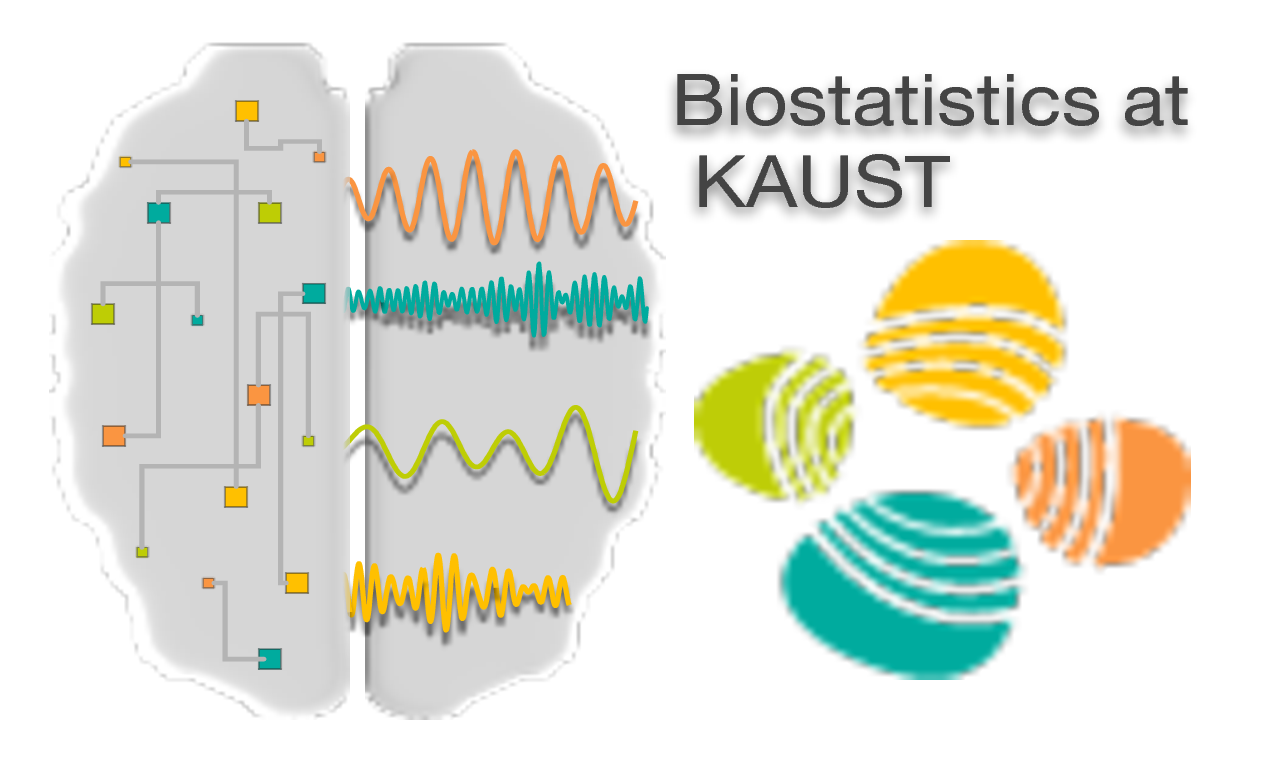
\includegraphics[height=1cm,width=2cm]{biostats_trans}}}
}%


\title{Time Series Analysis of Arctic Sea Ice}
\date{\today}
\author{Hector G. Flores Rodriguez}
\institute{KAUST Biostatistics}
\begin{document}
\maketitle

%\addtobeamertemplate{frametitle}{}{%
%\begin{textblock*}{100mm}(.85\textwidth,-1cm)
%	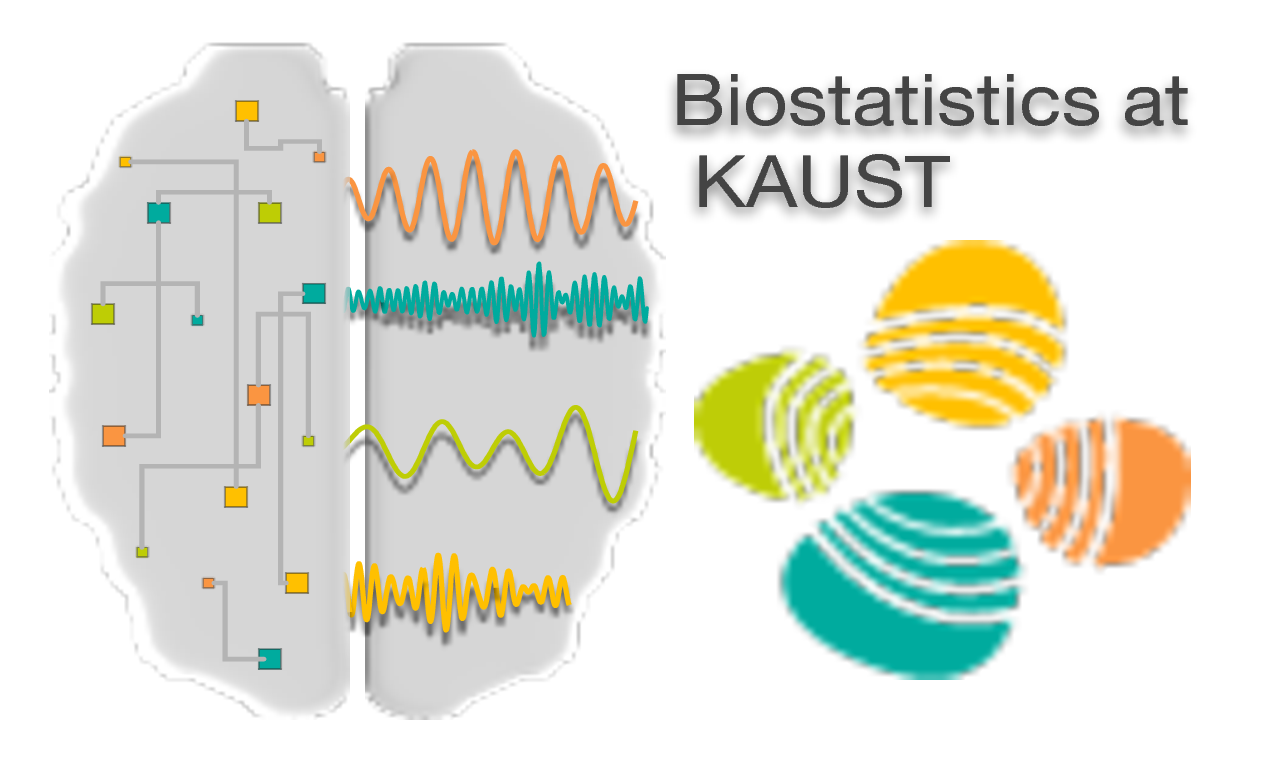
\includegraphics[height=1cm,width=2cm]{biostats.png}
%\end{textblock*}}

\begin{frame}{Table of contents}
  \setbeamertemplate{section in toc}[sections numbered]
  \tableofcontents[hideallsubsections]
\end{frame}
  
  
  
\section{Introduction}
\begin{frame}{Motivation}

The aim of this project is to further study and analyze Arctic Sea ice concentration. In particular, we want to investigate 

\begin{itemize}
\item any changes in the trend levels,
\item periodicities,
\item temporal correlation
\item spatial patterns of ice concentration
\end{itemize}
.
\end{frame}

%\begin{frame}{Background}
%The dataset is provided by the National Snow & Ice Data Center (NSIDC) in NetCDF4 format as shown in Table~\ref{data}.
%
%	\begin{table}[!htb]
%		\centering
%		\begin{tabular}{l|l}
%		\textbf{Variable} & \textbf{Description}                                                                                                                      		\\ \hline
%		latitude          & Latitude in degrees                                                                                                                       		\\ \hline
%		longitude         & Longitude in degrees (0 to 360)                                                                                                           		\\ \hline
%		seaice\_conc      & \begin{tabular}[c]{@{}l@{}}Sea ice concentration in percent 				with values\\ from 0 to 100, inclusive. Land is indicated by -1.\end{tabular} \\ 			\hline
%		seaice\_source    & \begin{tabular}[c]{@{}l@{}}Describes the source of the data 				for each month\\ of data beginning with January 1850\end{tabular}             \\ 			\hline
%		time              & \begin{tabular}[c]{@{}l@{}}Time of the data observation in 				days since\\ 1850-01-1 00:00:00\end{tabular}                                   \\ 	
%		\end{tabular}
%		\caption{Data set format}\label{data}
%		\end{table}
%\end{frame}

\begin{frame}{Yearly Averages}
Preliminary analysis of the data visually shows a decline in sea ice concentration levels towards the later part of the series.

	\begin{figure}[htbp]
		\centering
		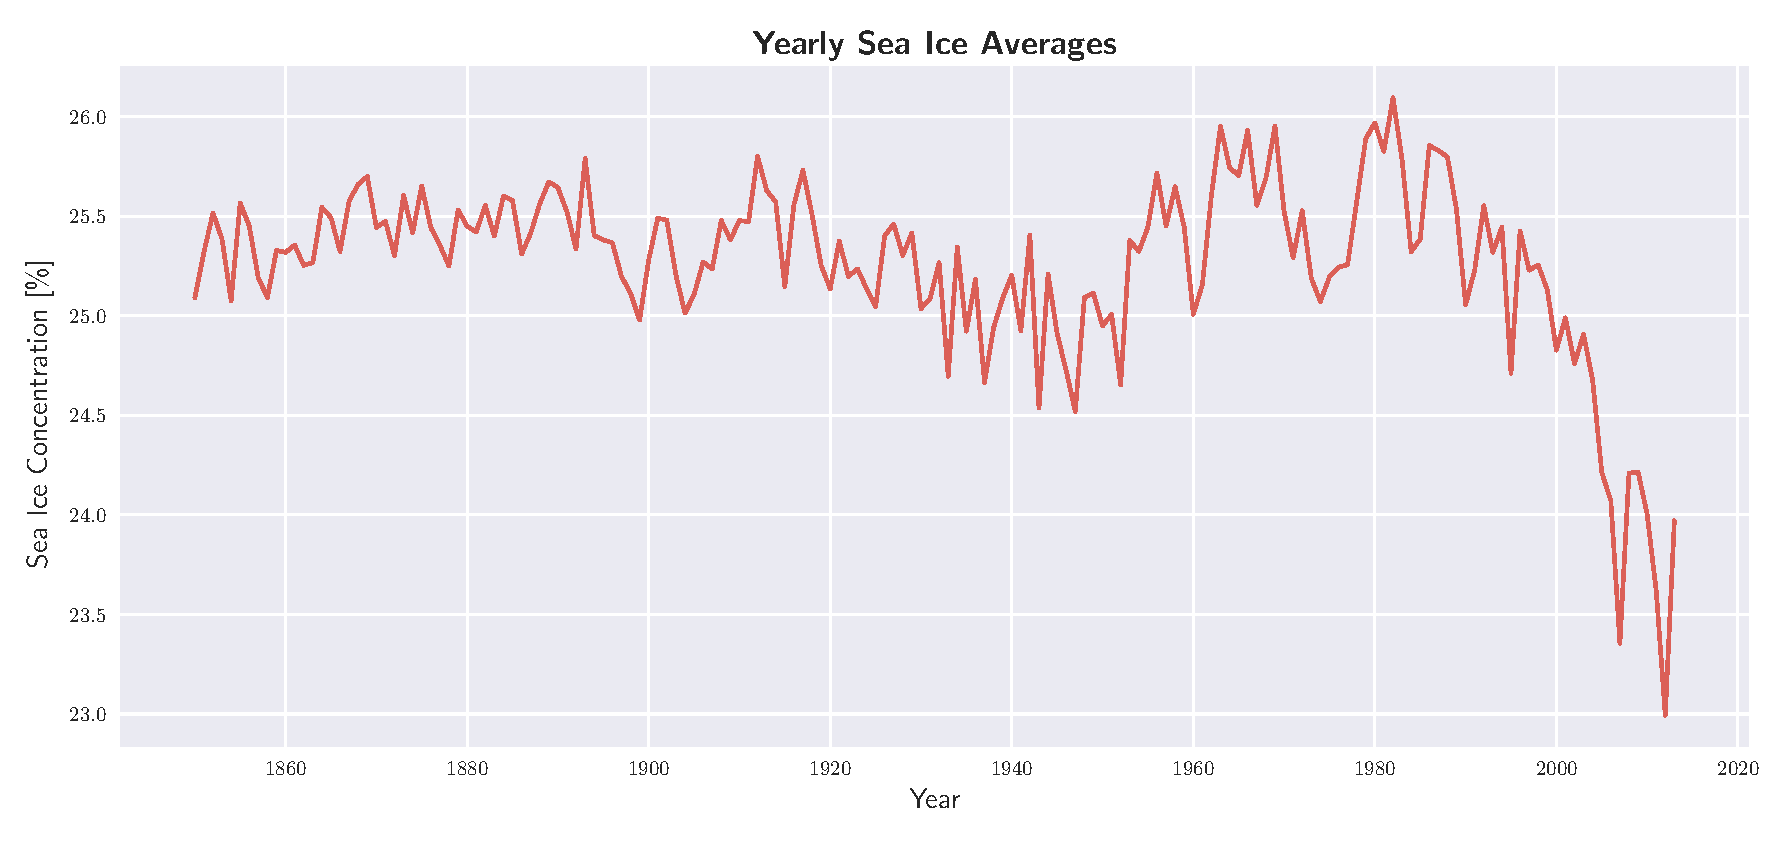
\includegraphics[scale=0.37]{yrly_avgs}
		\caption{Yearly sea ice concentration averages.}
	\end{figure}
\end{frame}

\begin{frame}{Seasonal Averages}
By decoupling the seasons, we can see that the winter (or colder) months are visually stable, whereas the summer (warmer) months show a greater decline.

	\begin{figure}[htbp]
		\centering
		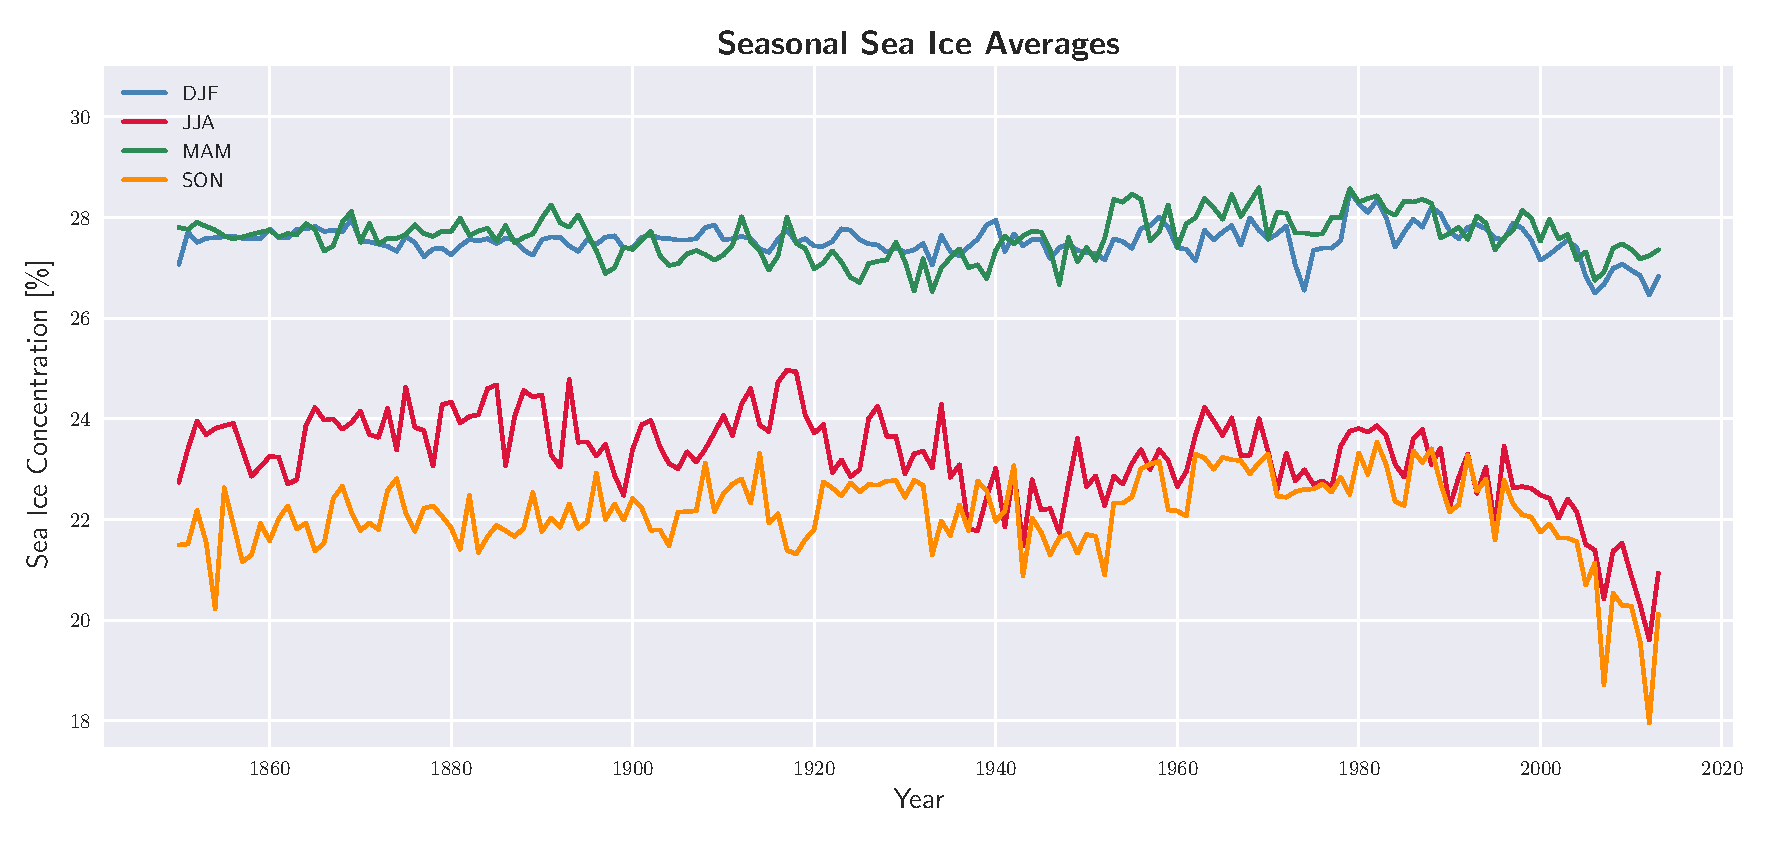
\includegraphics[scale=0.37]{seasonal_avgs}
		\caption{Seasonal sea ice concentration averages.}
	\end{figure}
\end{frame}

\section{Trend Analysis}
\begin{frame}{Trend Analysis}
The arctic sea ice data set introduces various climate phenomenas that greatly influences
the trend in the series.

Linear spline regression was used to determine significant changes in linear trends.
\end{frame}

\begin{frame}{Linear Splines}
We predefined our set of $K$ knots, $\xi_{1},...,\xi_{K}$, such that they lie on the $x$-axis and that they represent either:
\begin{itemize}
	\item Significant climate phenomena in time
	\item Significant visual change in the data
\end{itemize}

Define a linear spline with knot at $\xi_{k}$ to be:
$$(t-\xi_{k})_{+} = 
\begin{cases}
0, & \text{if $t < \xi_{t}$} \\
(t-\xi_{t}), & \text{if $t \geq \xi_{t}$}
\end{cases}$$

\begin{center}
\begin{tikzpicture}[scale=0.5]
\centering
\draw[->] (0,0) -- (4.8,0) node[right] {$x$}; 
\draw[->] (0,0) -- (0,2.7) node[above] {$y$};
\draw[blue] (0,0) -- (1,0);
\draw[->,blue] (1,0) node[black, below]{$\xi_1$} -- (2.5,1.5);
\draw[->,red] (2.5,0) node[black, below]{$\xi_2$} -- (4,1.5);
\draw[red] (1,0) -- (2.5,0);
\end{tikzpicture}
\end{center}
\end{frame}

\begin{frame}{Model}
Our model is then defined as

\setlength{\abovedisplayskip}{0pt}
\setlength{\belowdisplayskip}{0pt}
\begin{align*}
y_t &= \mu_t + s_t + \epsilon_t \\
\text{where,} \\
\mu_t &= \beta_0 + \beta_{1}t + \sum_{k=1}^{K}b_{k}(t-\xi_k)_{+} \\
s_t &= \sum_{j=1}^{m}[\alpha_{j}cos(2\pi\omega_{j}t) + \delta_{j}sin(2\pi\omega_{j}t)] \\
\end{align*}

$y_t$ are the observations, $\mu_t$ denotes the piecewise linear trend, $s_t$ is the seasonality component, and $\epsilon_t$ is the random component that accounts for temporal correlation in $\{y_t\}$.

\\

\end{frame}

\begin{frame}{Summer Trends}
The year 1997 was selected with a significance level, $\alpha=0.05$, after several multiple comparison tests were made.
	\begin{figure}[htbp]
		\centering
		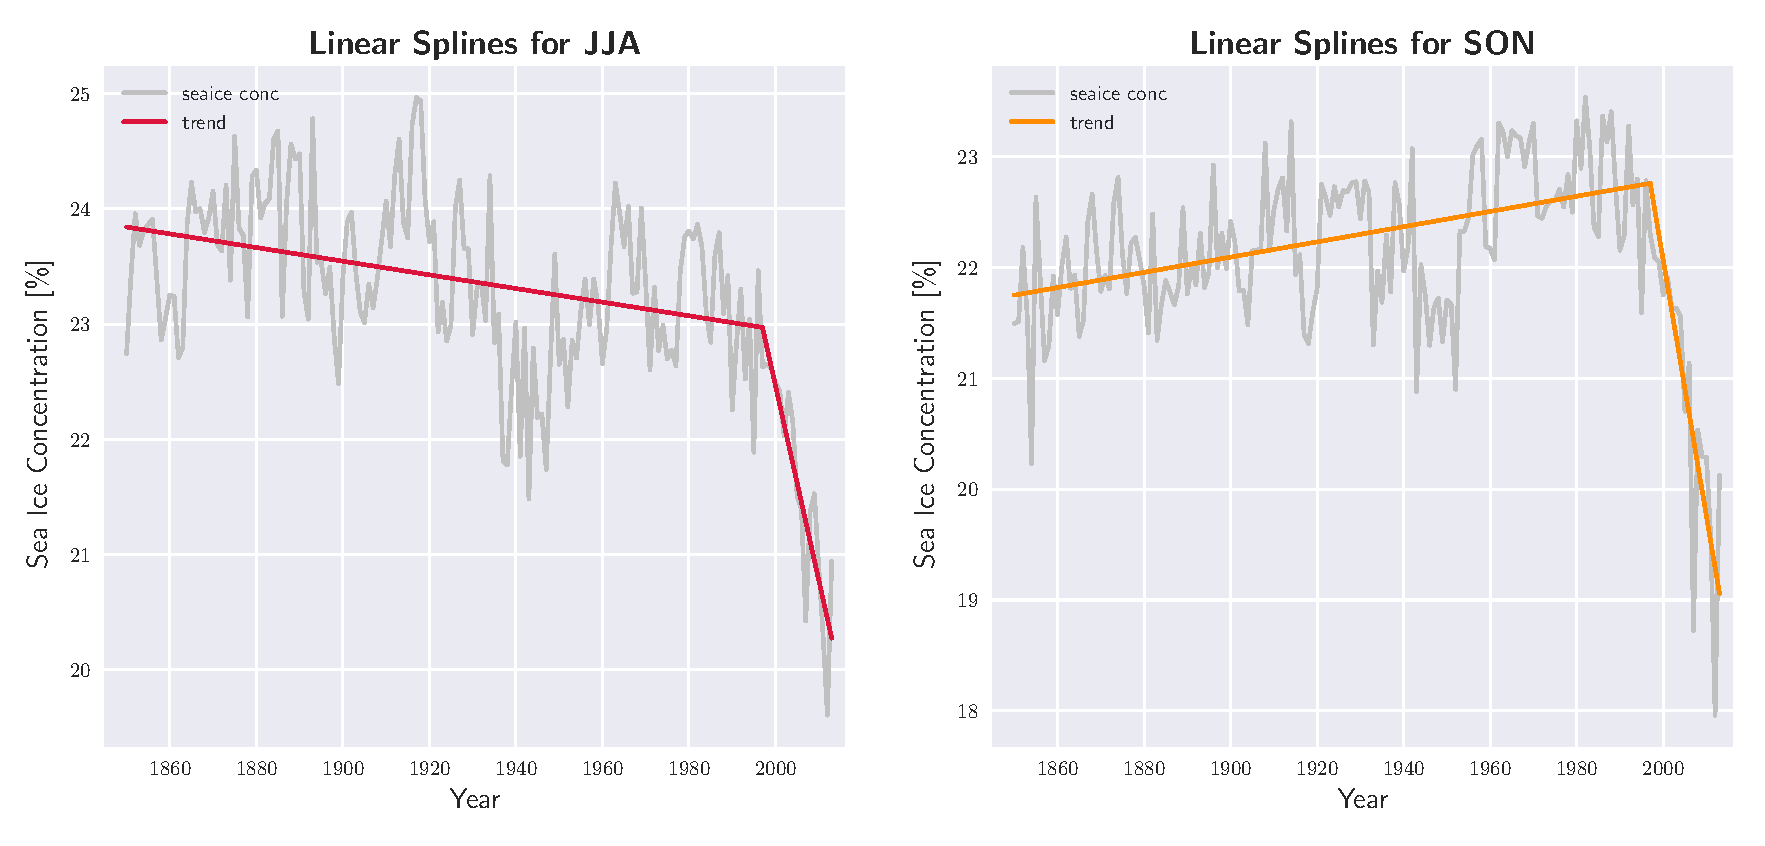
\includegraphics[scale=0.37]{summer_splines}
		\caption{Linear spline regression fit for summer seasons.}
	\end{figure}
\end{frame}

\begin{frame}{Winter Trends}
The year 1997 was selected for the months: December, January, February. Whereas, 1933 and 1979, were selected for the months: March, April, May.
	\begin{figure}[htbp]
		\centering
		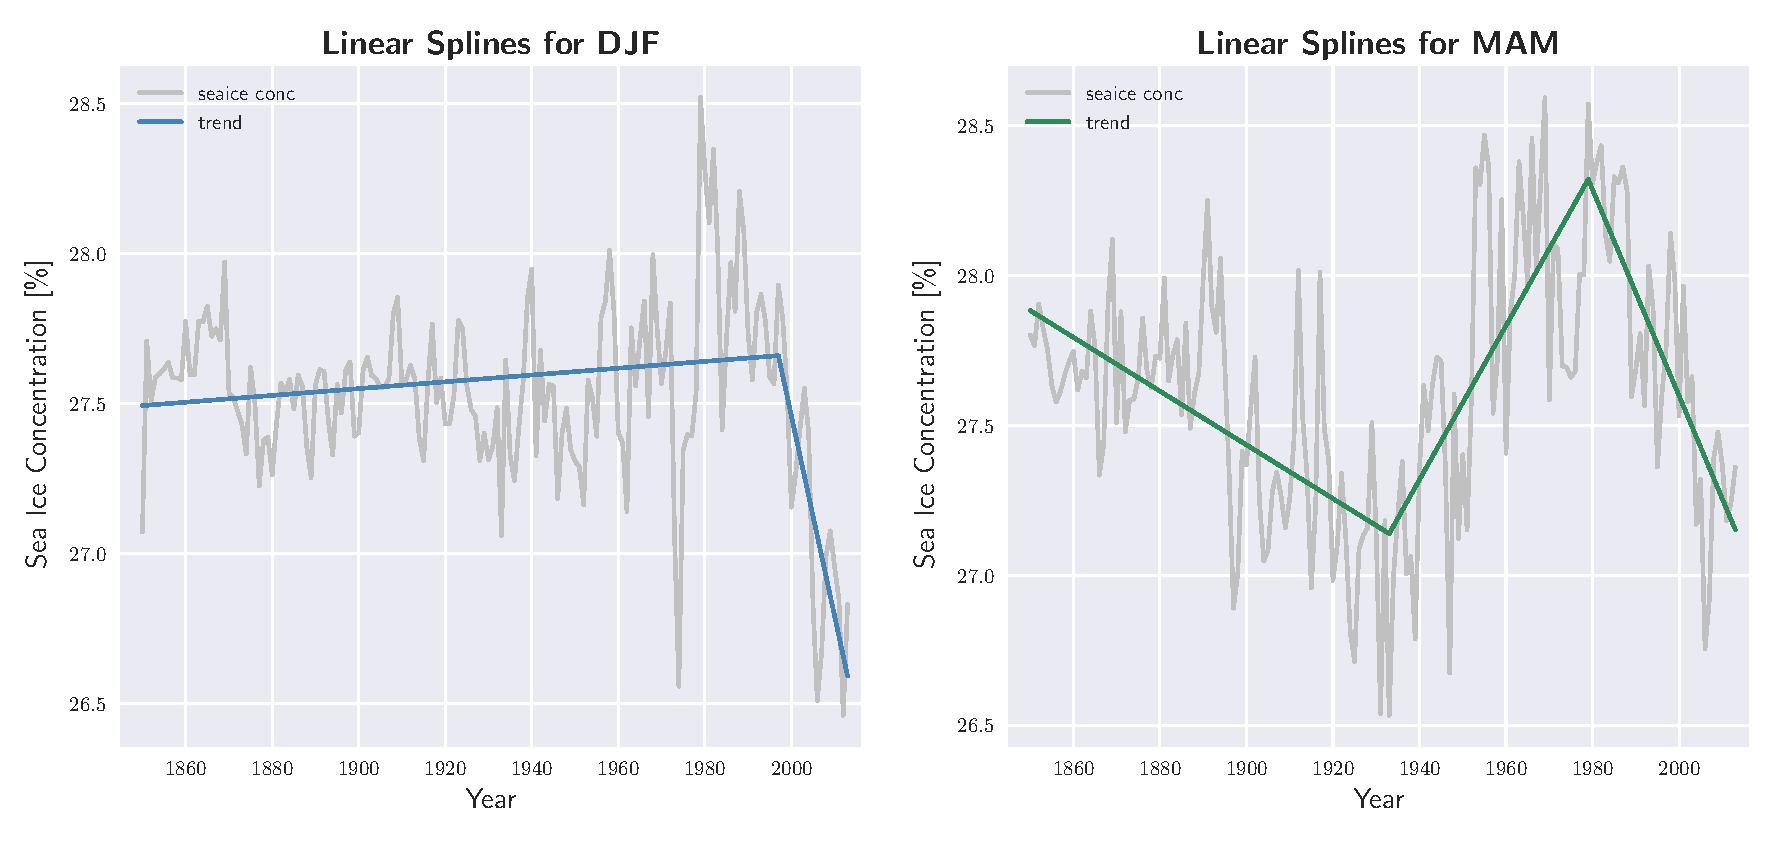
\includegraphics[scale=0.37]{winter_splines}
		\caption{Linear spline regression fit for winter seasons.}
	\end{figure}
\end{frame}

\begin{frame}{Detrending}
By removing the piecewise regression line, we can study periodicity and temporal correlation since 
$$e_t \approx s_t + \epsilon_t$$

Further analysis are performed on the detrended series, $e_t$, which is be expressed as

$$e_t = y_t - \hat{\mu_t}$$

where $\hat{\mu_t}$ is computed using Iteratively Reweighted Least Squares (IRLS).

\end{frame}

%\begin{frame}{Test For Stationarity}
%The Augmented Dickey-Fuller test was employed to determine the stationarity of our series
%\end{frame}

\section{Spectral Analysis}

\begin{frame}{Spectral Analysis Purpose}
The purpose of spectral analysis is to study oscilations present in the time series. In particular, we shall identify periodicity trends in the ice concentration.
\end{frame}

\begin{frame}{Spectral Density Estimation}
\setlength{\abovedisplayskip}{0pt}
\setlength{\belowdisplayskip}{0pt}
\setlength{\abovedisplayshortskip}{0pt}
\setlength{\belowdisplayshortskip}{0pt}

An estimate of the spectral density is obtained using Welch's Method

\setlength{\abovedisplayskip}{0pt}
\setlength{\belowdisplayskip}{0pt}
\begin{itemize}
\item the residuals, $e_t$, are split into $K$ overlapping segments of length $L$
\item apply Hanning window $w(n) = \frac{1}{2}({1} - {\cos{(2\pi\frac{n}{N})}})$ to segments
\item all $K$ periodograms are averaged \\
\setlength{\mathindent}{0pt}
\setlength{\abovedisplayskip}{0pt}
\setlength{\belowdisplayskip}{0pt}
\begin{align*}
\hat{P}_{welch}(e^{j\omega}) &= \frac{1}{K} \sum_{k=1}^{K} \hat{P}_{y}^{(k)}(e^{j\omega})
\: \text{  where,} \\
\hat{P}_{y}^{(k)} &= 
			\frac{1}{N} \sum_{n=0}^{L-1} \left|w(n)y^{(k)}(n) e^{-j \omega n}\right|^{2}
\end{align*}
\end{itemize}


\end{frame}
  
\begin{frame}{Summer PSD}
	\begin{figure}[htbp]
		\centering
		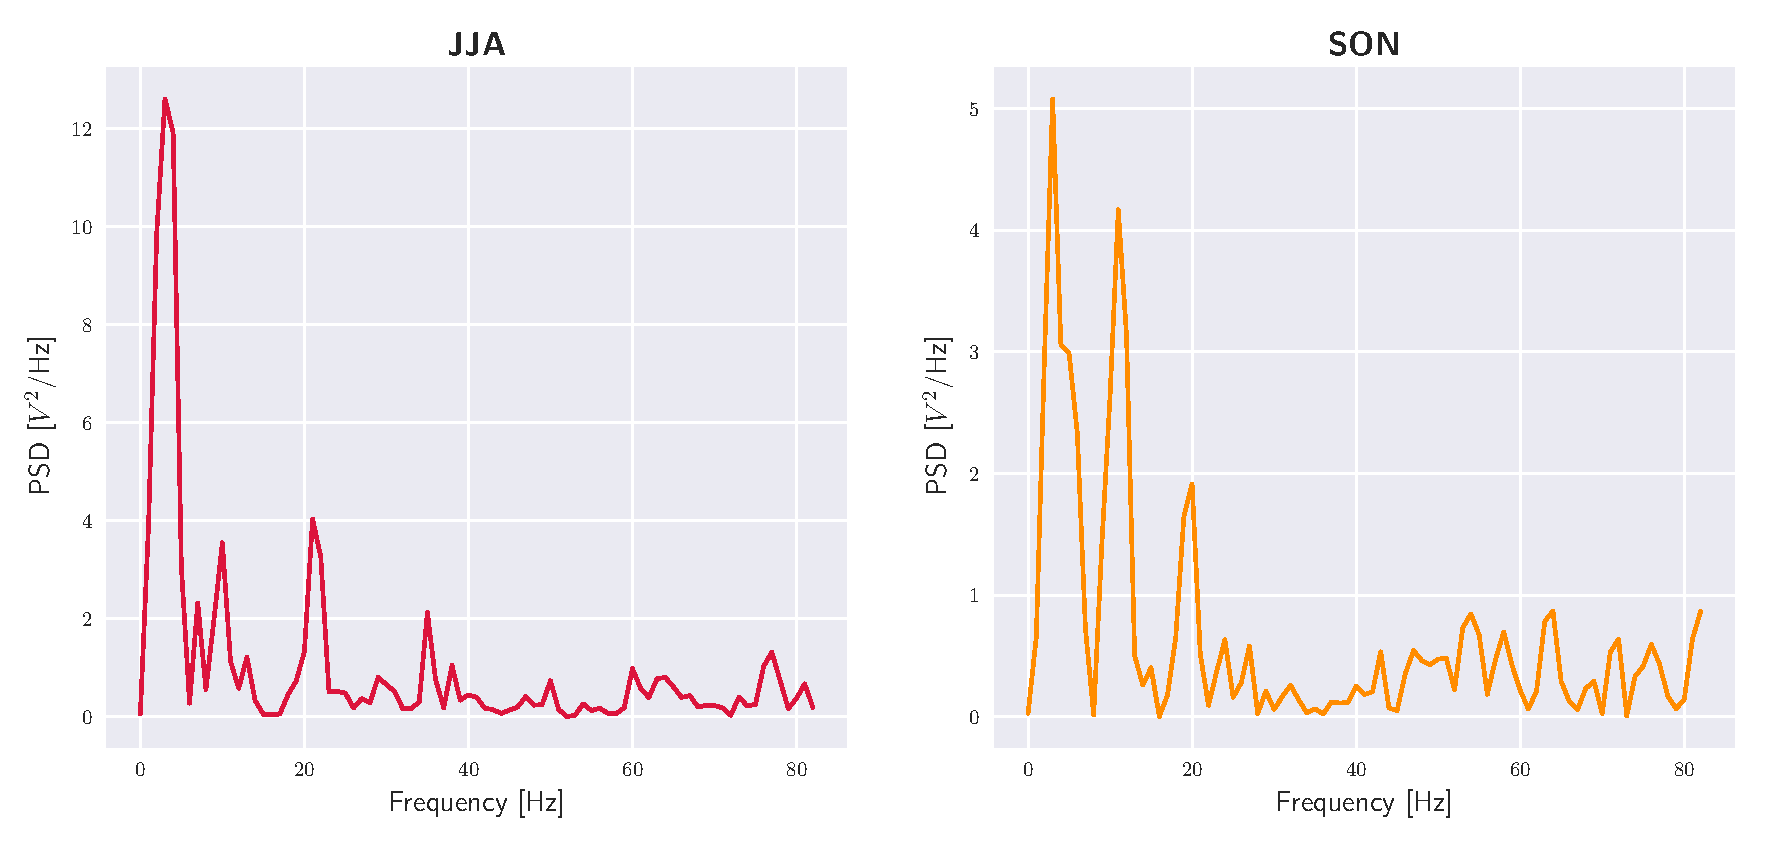
\includegraphics[scale=0.37]{summer_psd}
		\caption{Estimated spectral density for summer seasons.}
	\end{figure}
\end{frame}

\begin{frame}{Winter PSD}
	\begin{figure}[htbp]
		\centering
		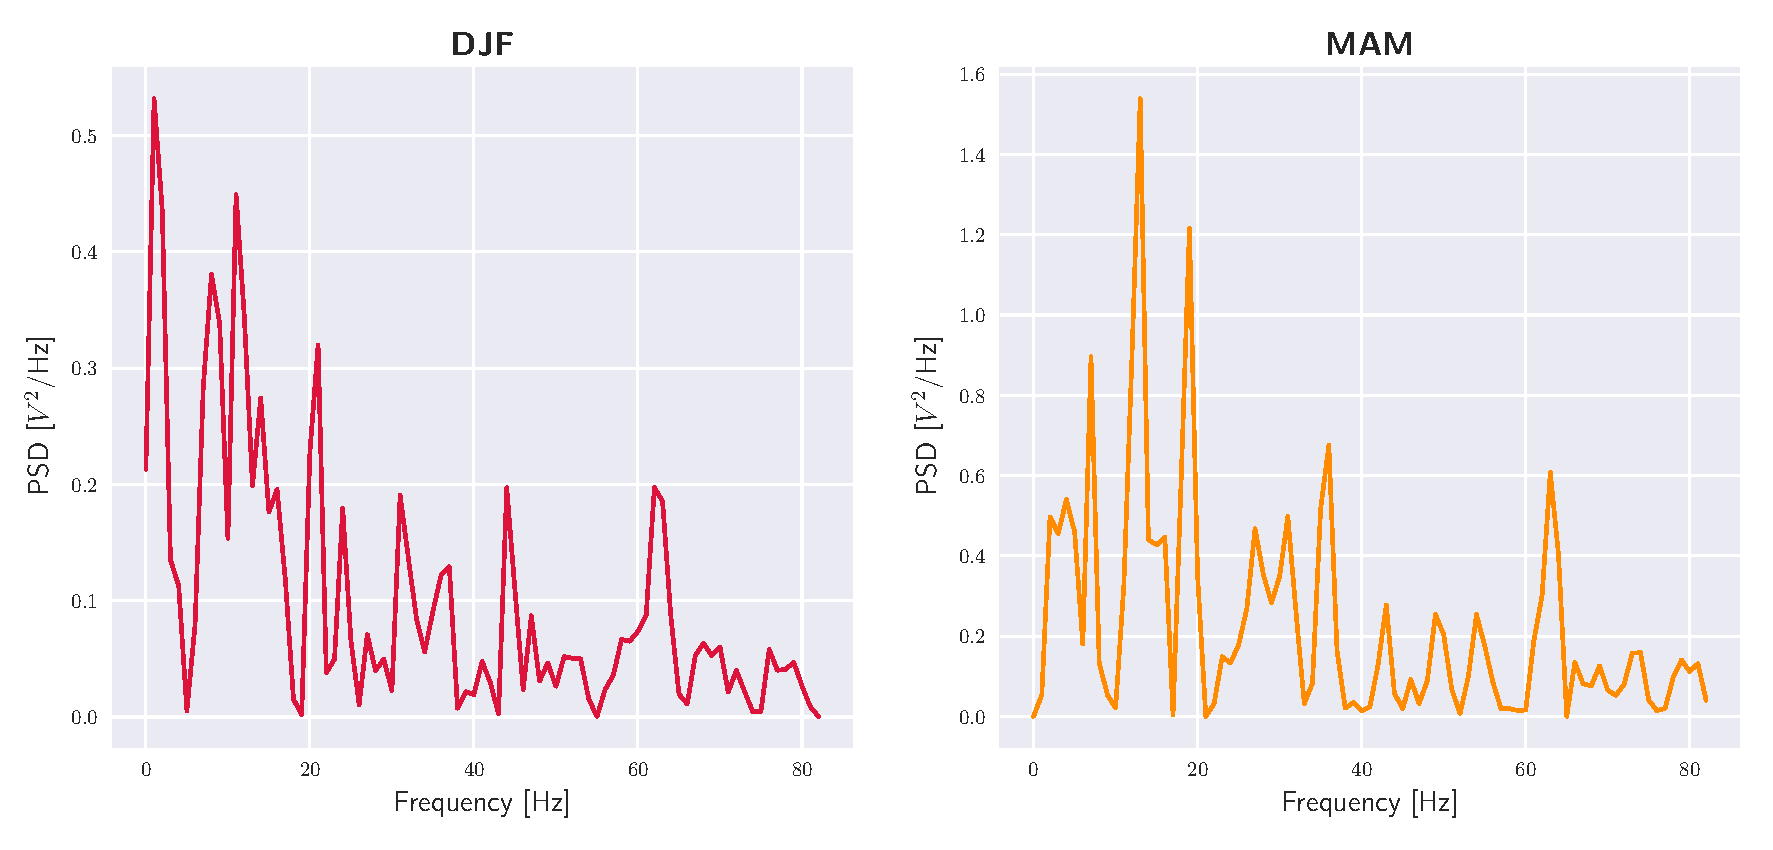
\includegraphics[scale=0.37]{winter_psd}
		\caption{Estimated spectral density for winter seasons.}
	\end{figure}
\end{frame}

\begin{frame}{Harmonic Regression}
To capture seasonal patterns, we consider the following model,

$$
s_t = 
\sum_{j=1}^{m}[\alpha_{j}sin(2\pi\omega_{j}t)+\delta_{j}cos(2\pi\omega_{j}t)]
$$

where coefficients $\alpha_j$ and $\delta_j$ are estimated but the frequencies
$\omega_j$ are obtained from the power spectrum estimate.

\end{frame}

\begin{frame}{Harmonic Frequencies}
The harmonic components are chosen at a significance level, $\alpha=0.05$, and are shown in Table~\ref{frequencies}

	\begin{table}[!htb]
	\centering
	\begin{tabular}{l|l|l|l}
	\textbf{JJA}       & \textbf{SON}     & \textbf{DJF}     & \textbf{MAM} \\ \hline
	$sin(\omega_{3}t)  & sin(\omega_{3}t) & cos(\omega_{2}t) & sin(\omega_{2}t)$   \\
	$cos(\omega_{3}t)  & cos(\omega_{3}t) & sin(\omega_{4}t) & cos(\omega_{2}t)$   \\
	$sin(\omega_{10}t) &                  & cos(\omega_{4}t) & sin(\omega_{13}t)$   \\
	$cos(\omega_{10}t) &                  &                  &                  $   \\
	\end{tabular}
	\caption{Harmonic frequencies computed from periodogram.}\label{frequencies}
	\end{table}
\end{frame}

\section{AR Model}
\begin{frame}{Model Selection}

\begin{itemize}
\item Determine initial set of ARMA models using both Autocorrelation Function (ACF) and Partial Autocorrelation Function (PACF)
\item Select the best model according to Akaike information criterion (AIC) and  Bayesian information criterion (BIC)
\end{itemize}

\end{frame}

\begin{frame}{JJA ACF and PACF}
	\begin{figure}[htbp]
		\centering
		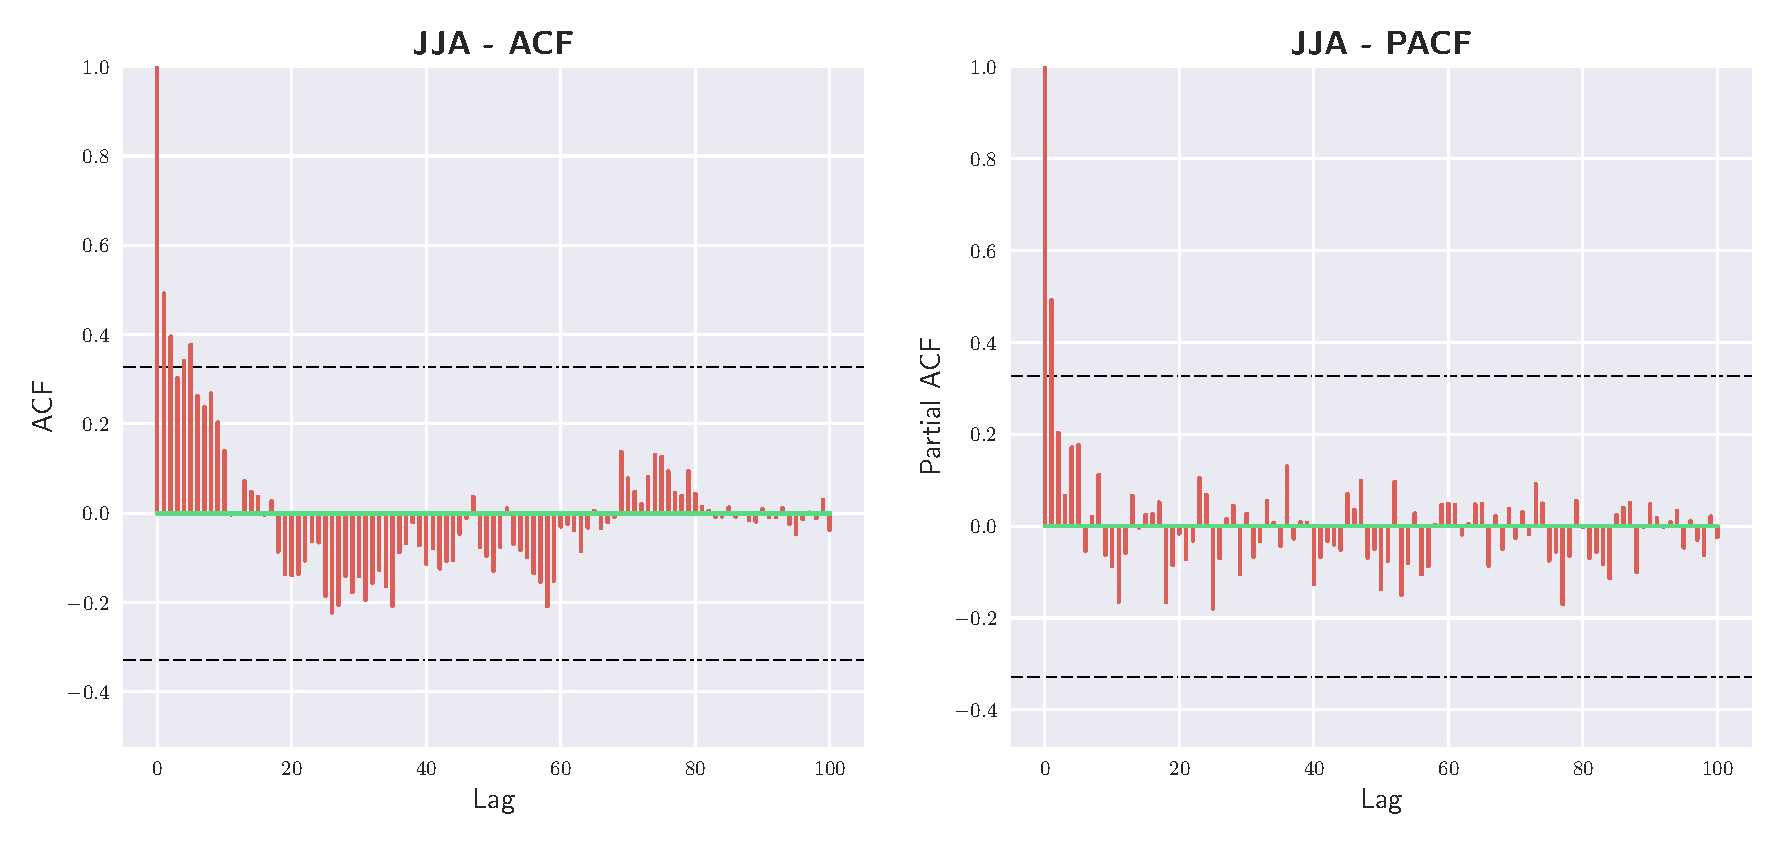
\includegraphics[scale=0.37]{jja_acf}
		\caption{JJA ACF and PACF plots.}
	\end{figure}
\end{frame}

\begin{frame}{SON ACF and PACF}
	\begin{figure}[htbp]
		\centering
		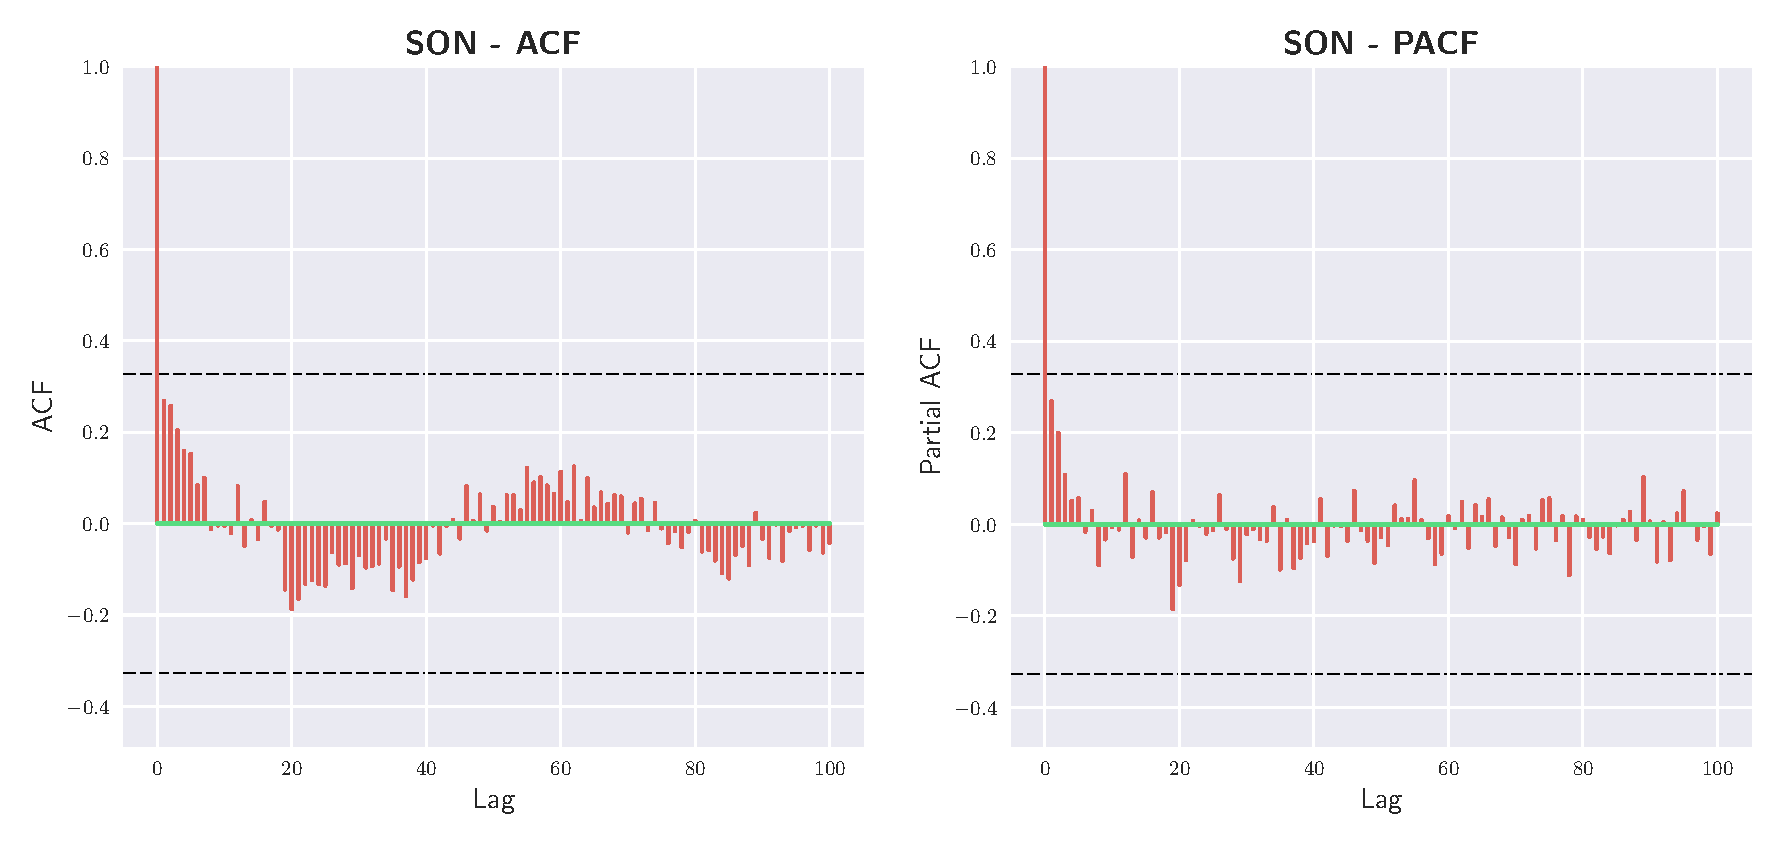
\includegraphics[scale=0.37]{son_acf}
		\caption{SON ACF and PACF plots.}
	\end{figure}
\end{frame}

\begin{frame}{DJF ACF and PACF}
	\begin{figure}[htbp]
		\centering
		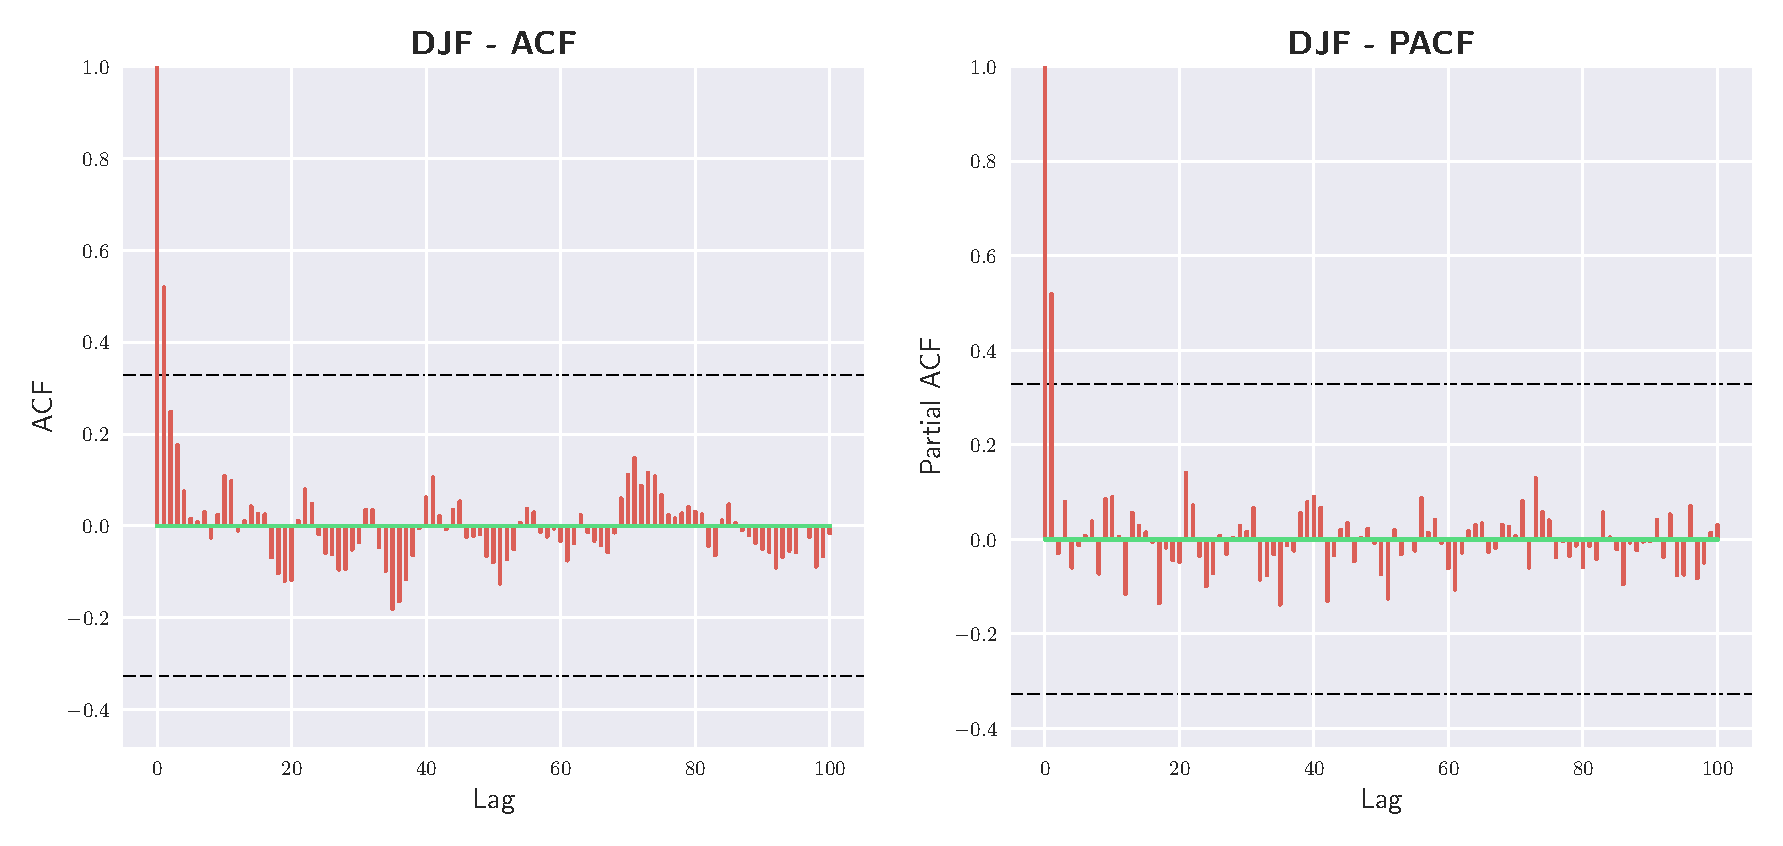
\includegraphics[scale=0.37]{djf_acf}
		\caption{DJF ACF and PACF plots.}
	\end{figure}
\end{frame}

\begin{frame}{MAM ACF and PACF}
	\begin{figure}[htbp]
		\centering
		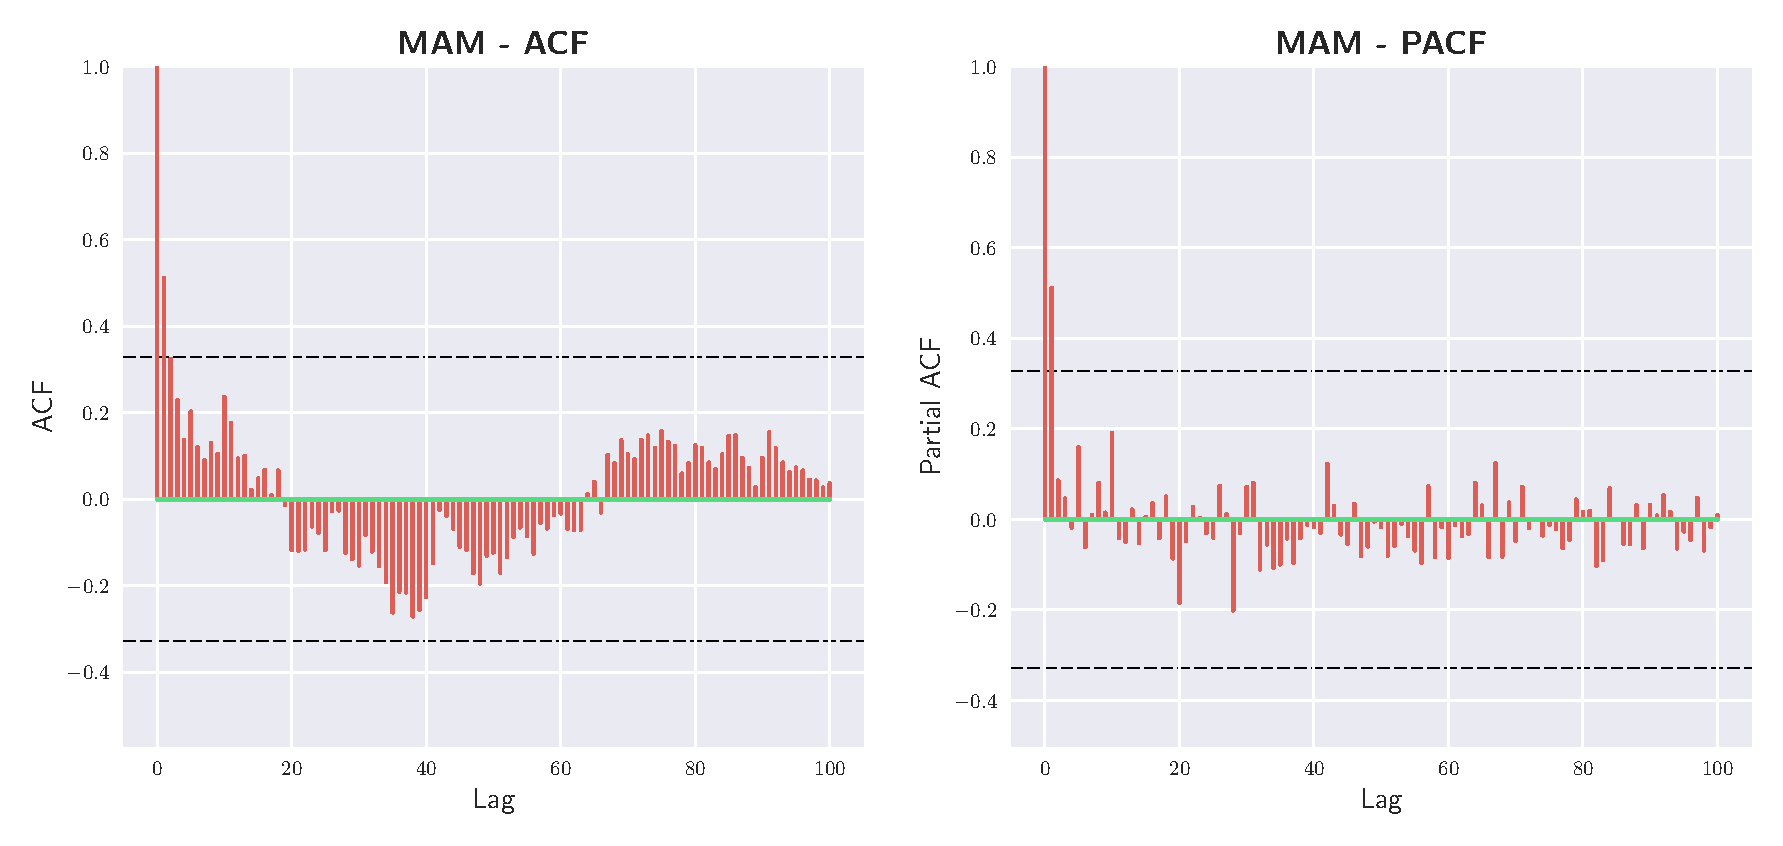
\includegraphics[scale=0.37]{mam_acf}
		\caption{MAM ACF and PACF plots.}
	\end{figure}
\end{frame}

\section{Results}
\begin{frame}{Whiteness Testing}
To ensure our models were appropriate  (i.e., good estimates of  trend and periodicity), we tested the residuals for "whiteness" by:
  \begin{itemize}
    \item Analyzing the ACFs and PACFs
    \item Performing Ljung-Box test for up to 10 lags
    \item QQ plot for normality
\end{itemize}
\end{frame}

\begin{frame}{JJA Residuals}
	\begin{figure}[htbp]
		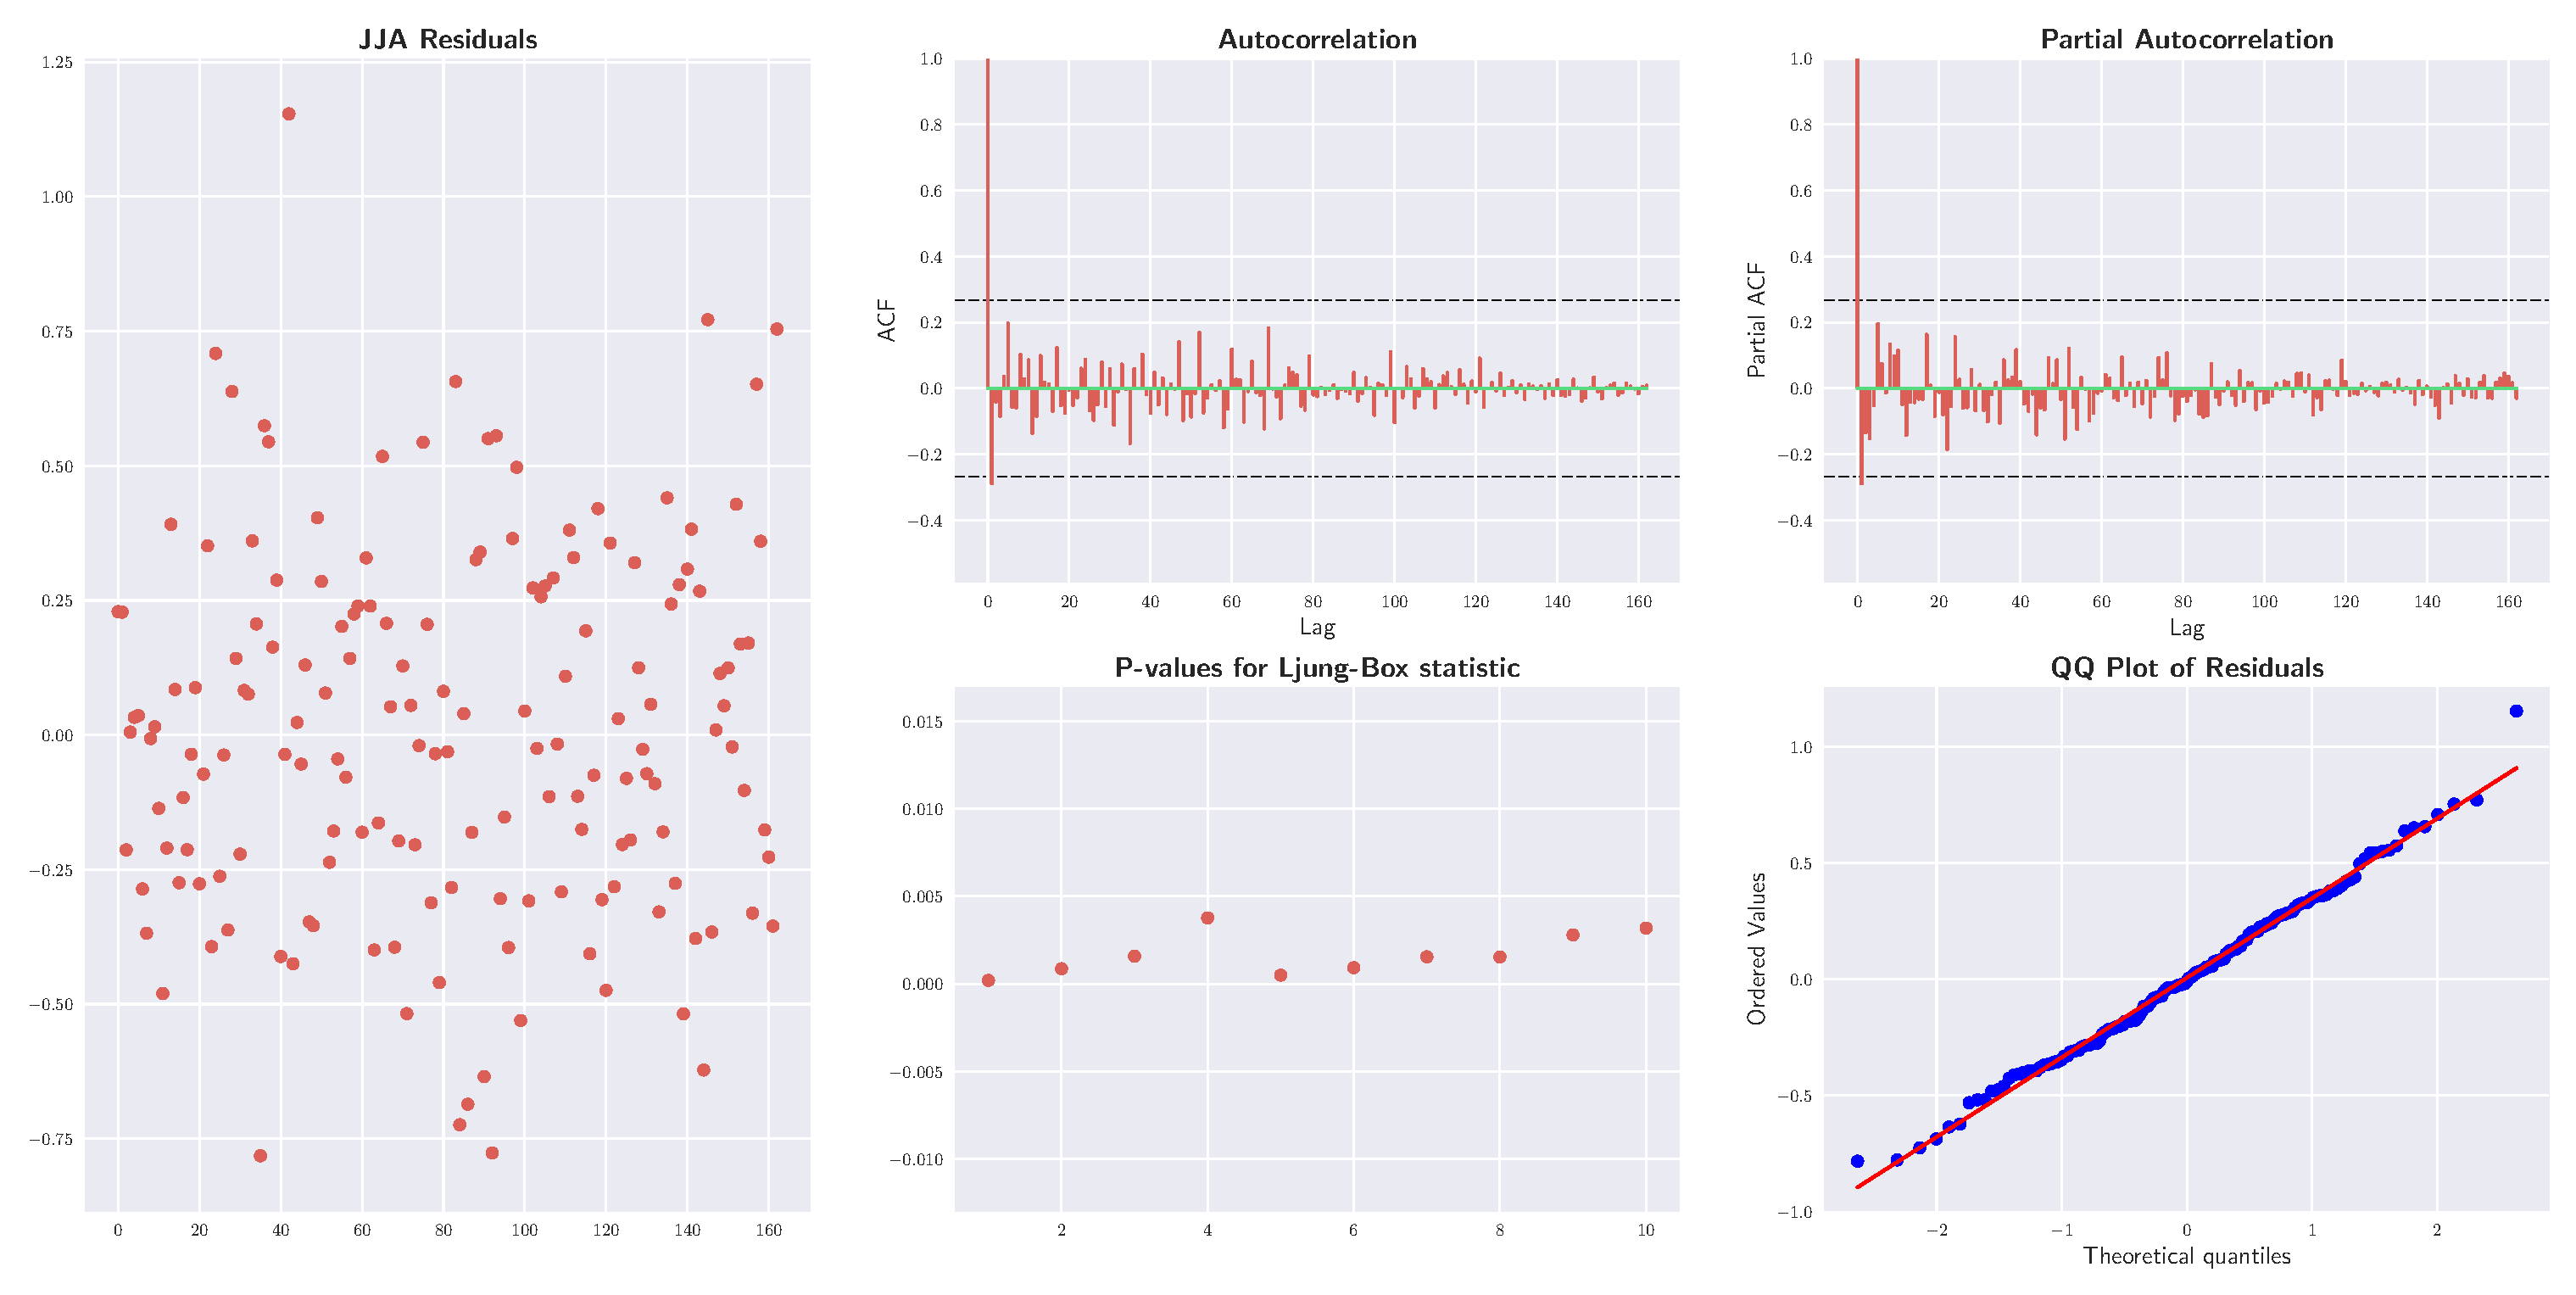
\includegraphics[scale=0.225,left]{jja_res}
		\caption{JJA residuals diagnostic tests.}
	\end{figure}
\end{frame}

\begin{frame}{SON Residuals}
	\begin{figure}[htbp]
		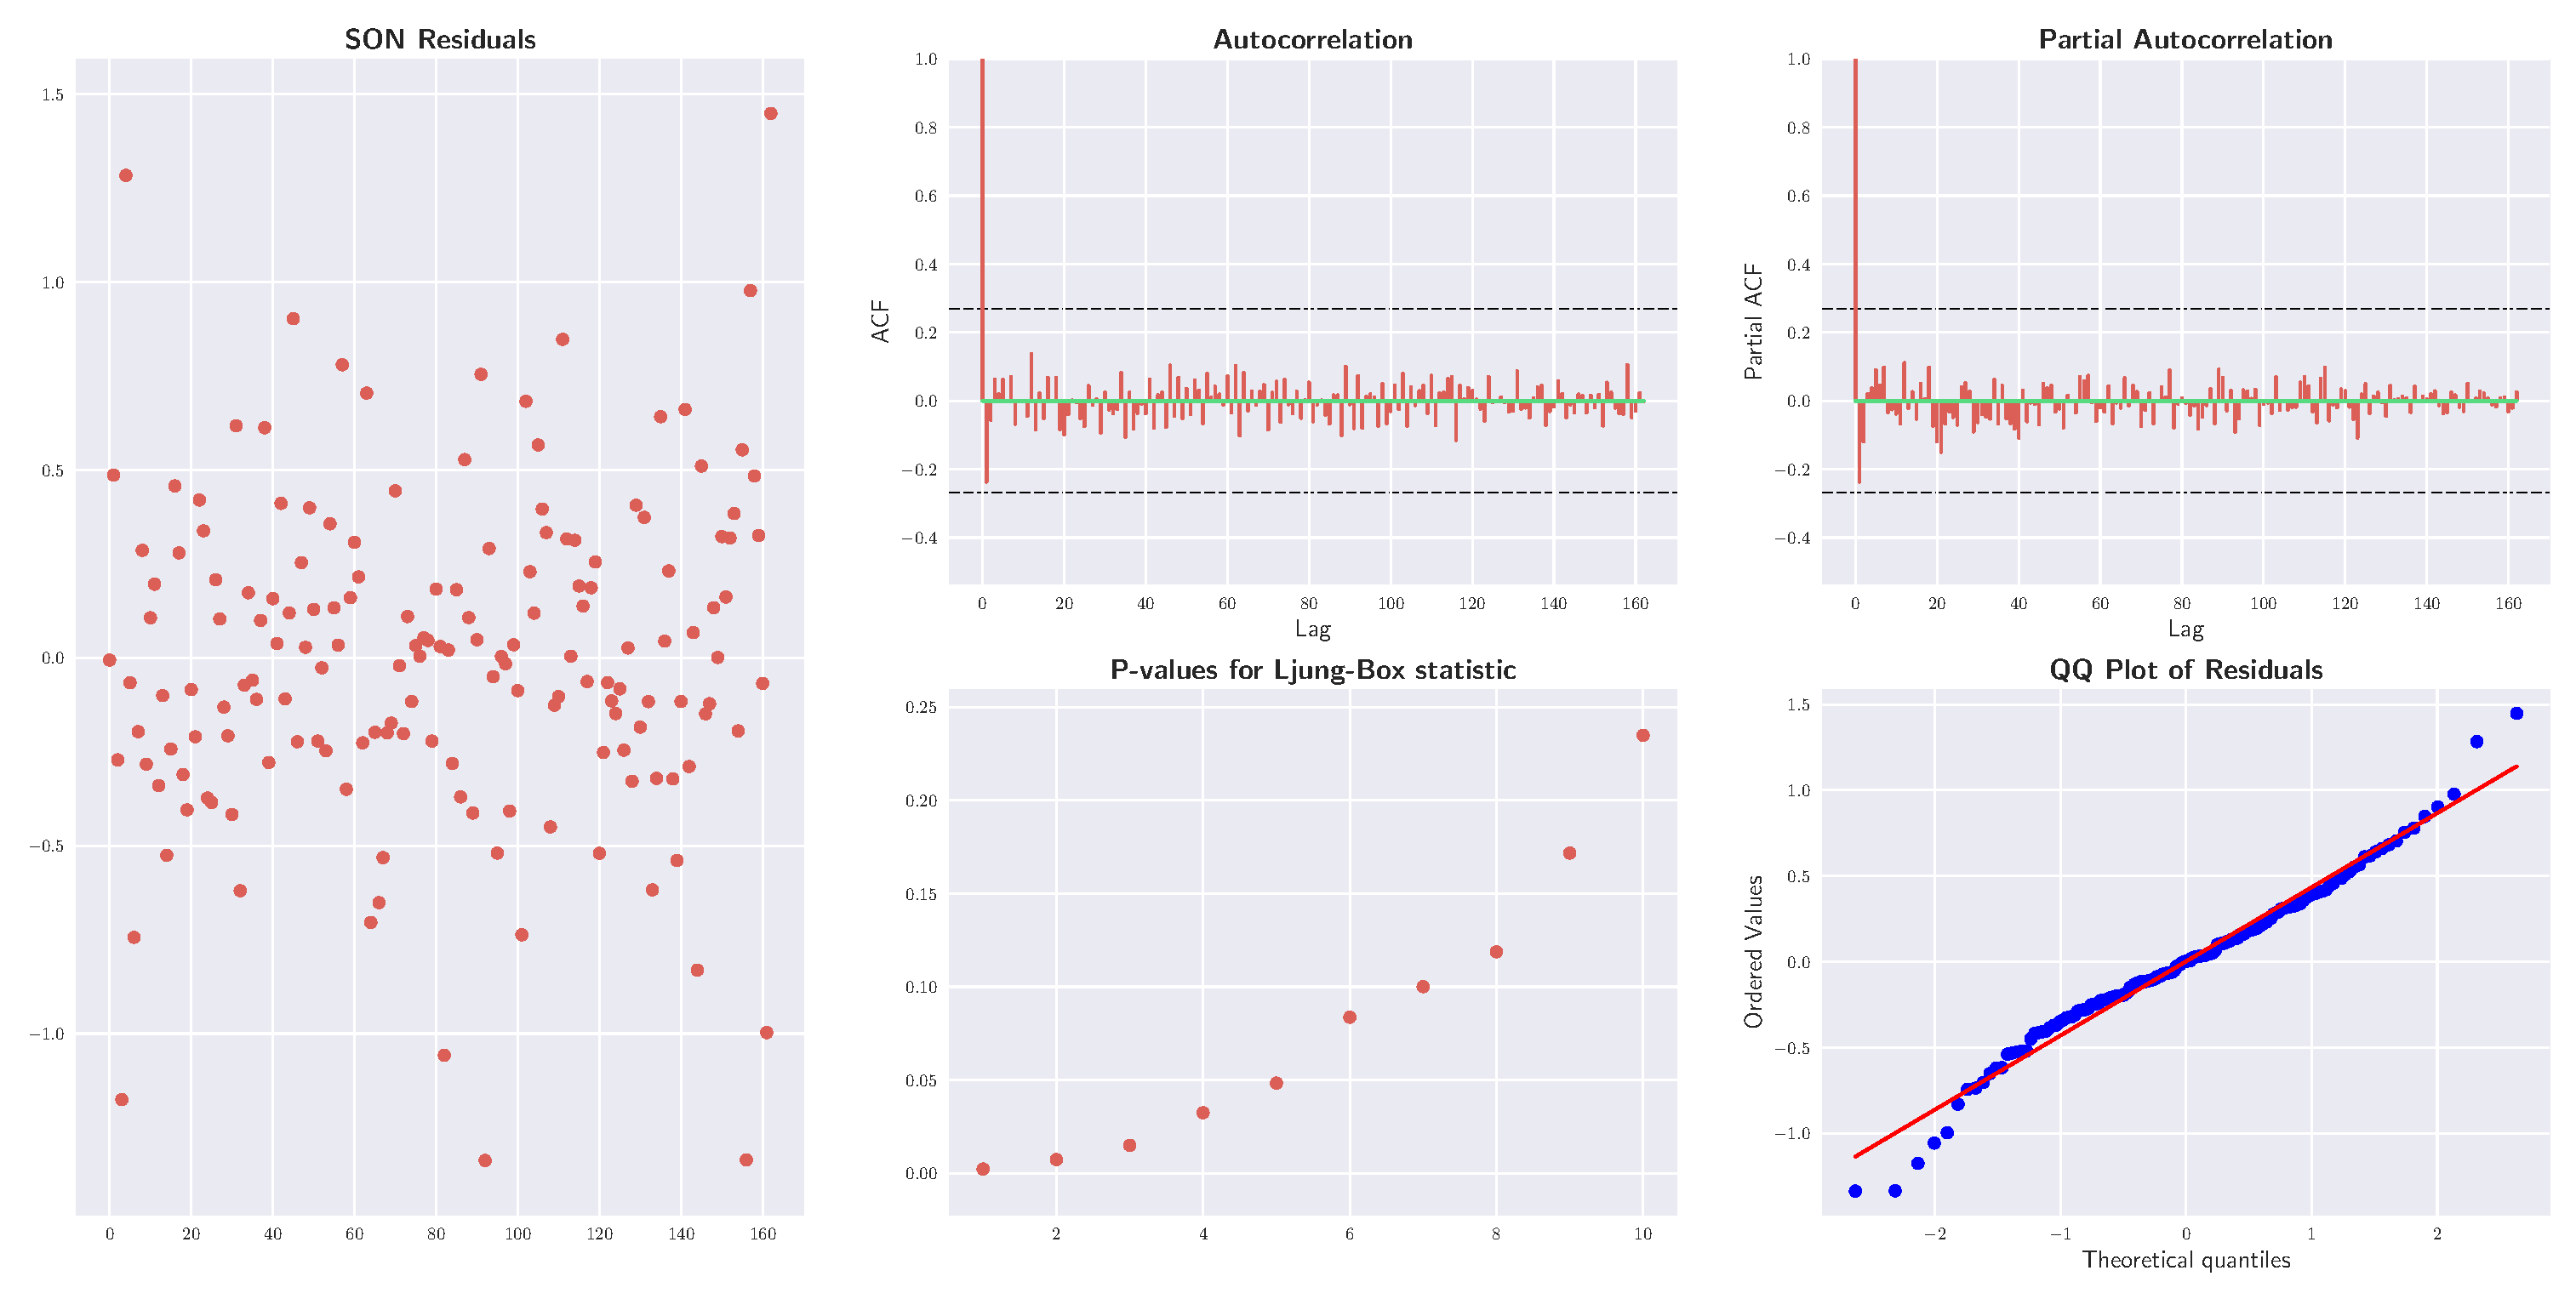
\includegraphics[scale=0.225,left]{son_res}
		\caption{SON residuals diagnostic tests.}
	\end{figure}
\end{frame}

\begin{frame}{DJF Residuals}
	\begin{figure}[htbp]
		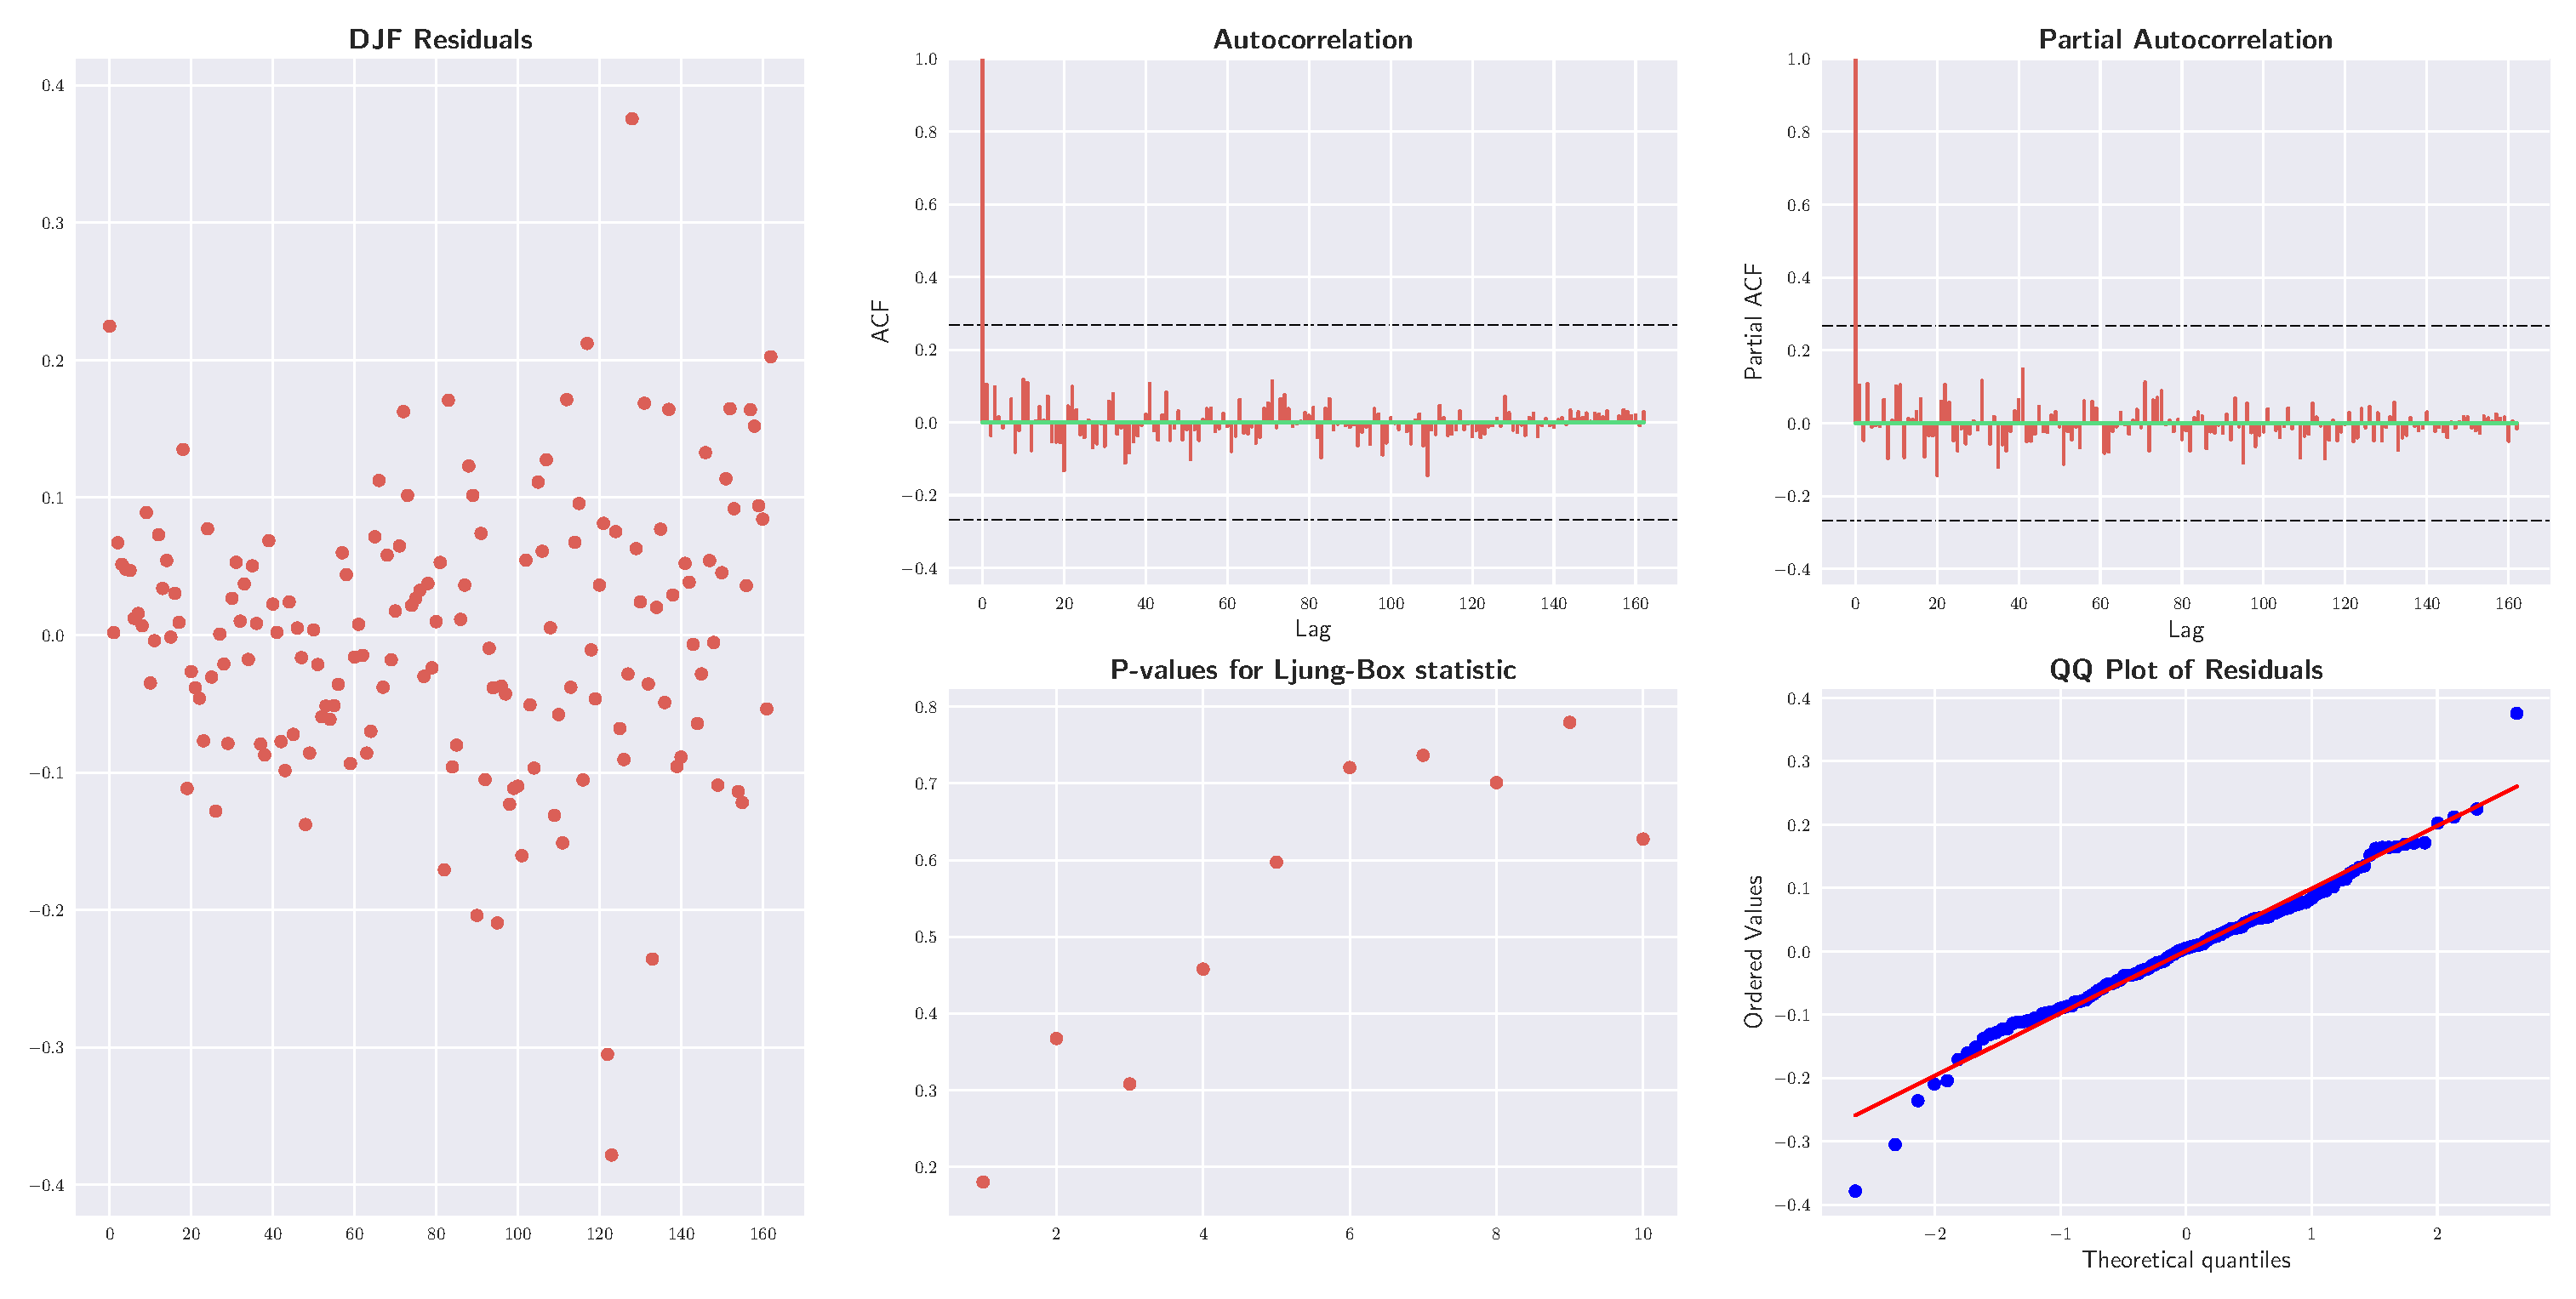
\includegraphics[scale=0.225,left]{djf_res}
		\caption{DJF residuals diagnostic tests.}
	\end{figure}
\end{frame}

\begin{frame}{MAM Residuals}
	\begin{figure}[htbp]
		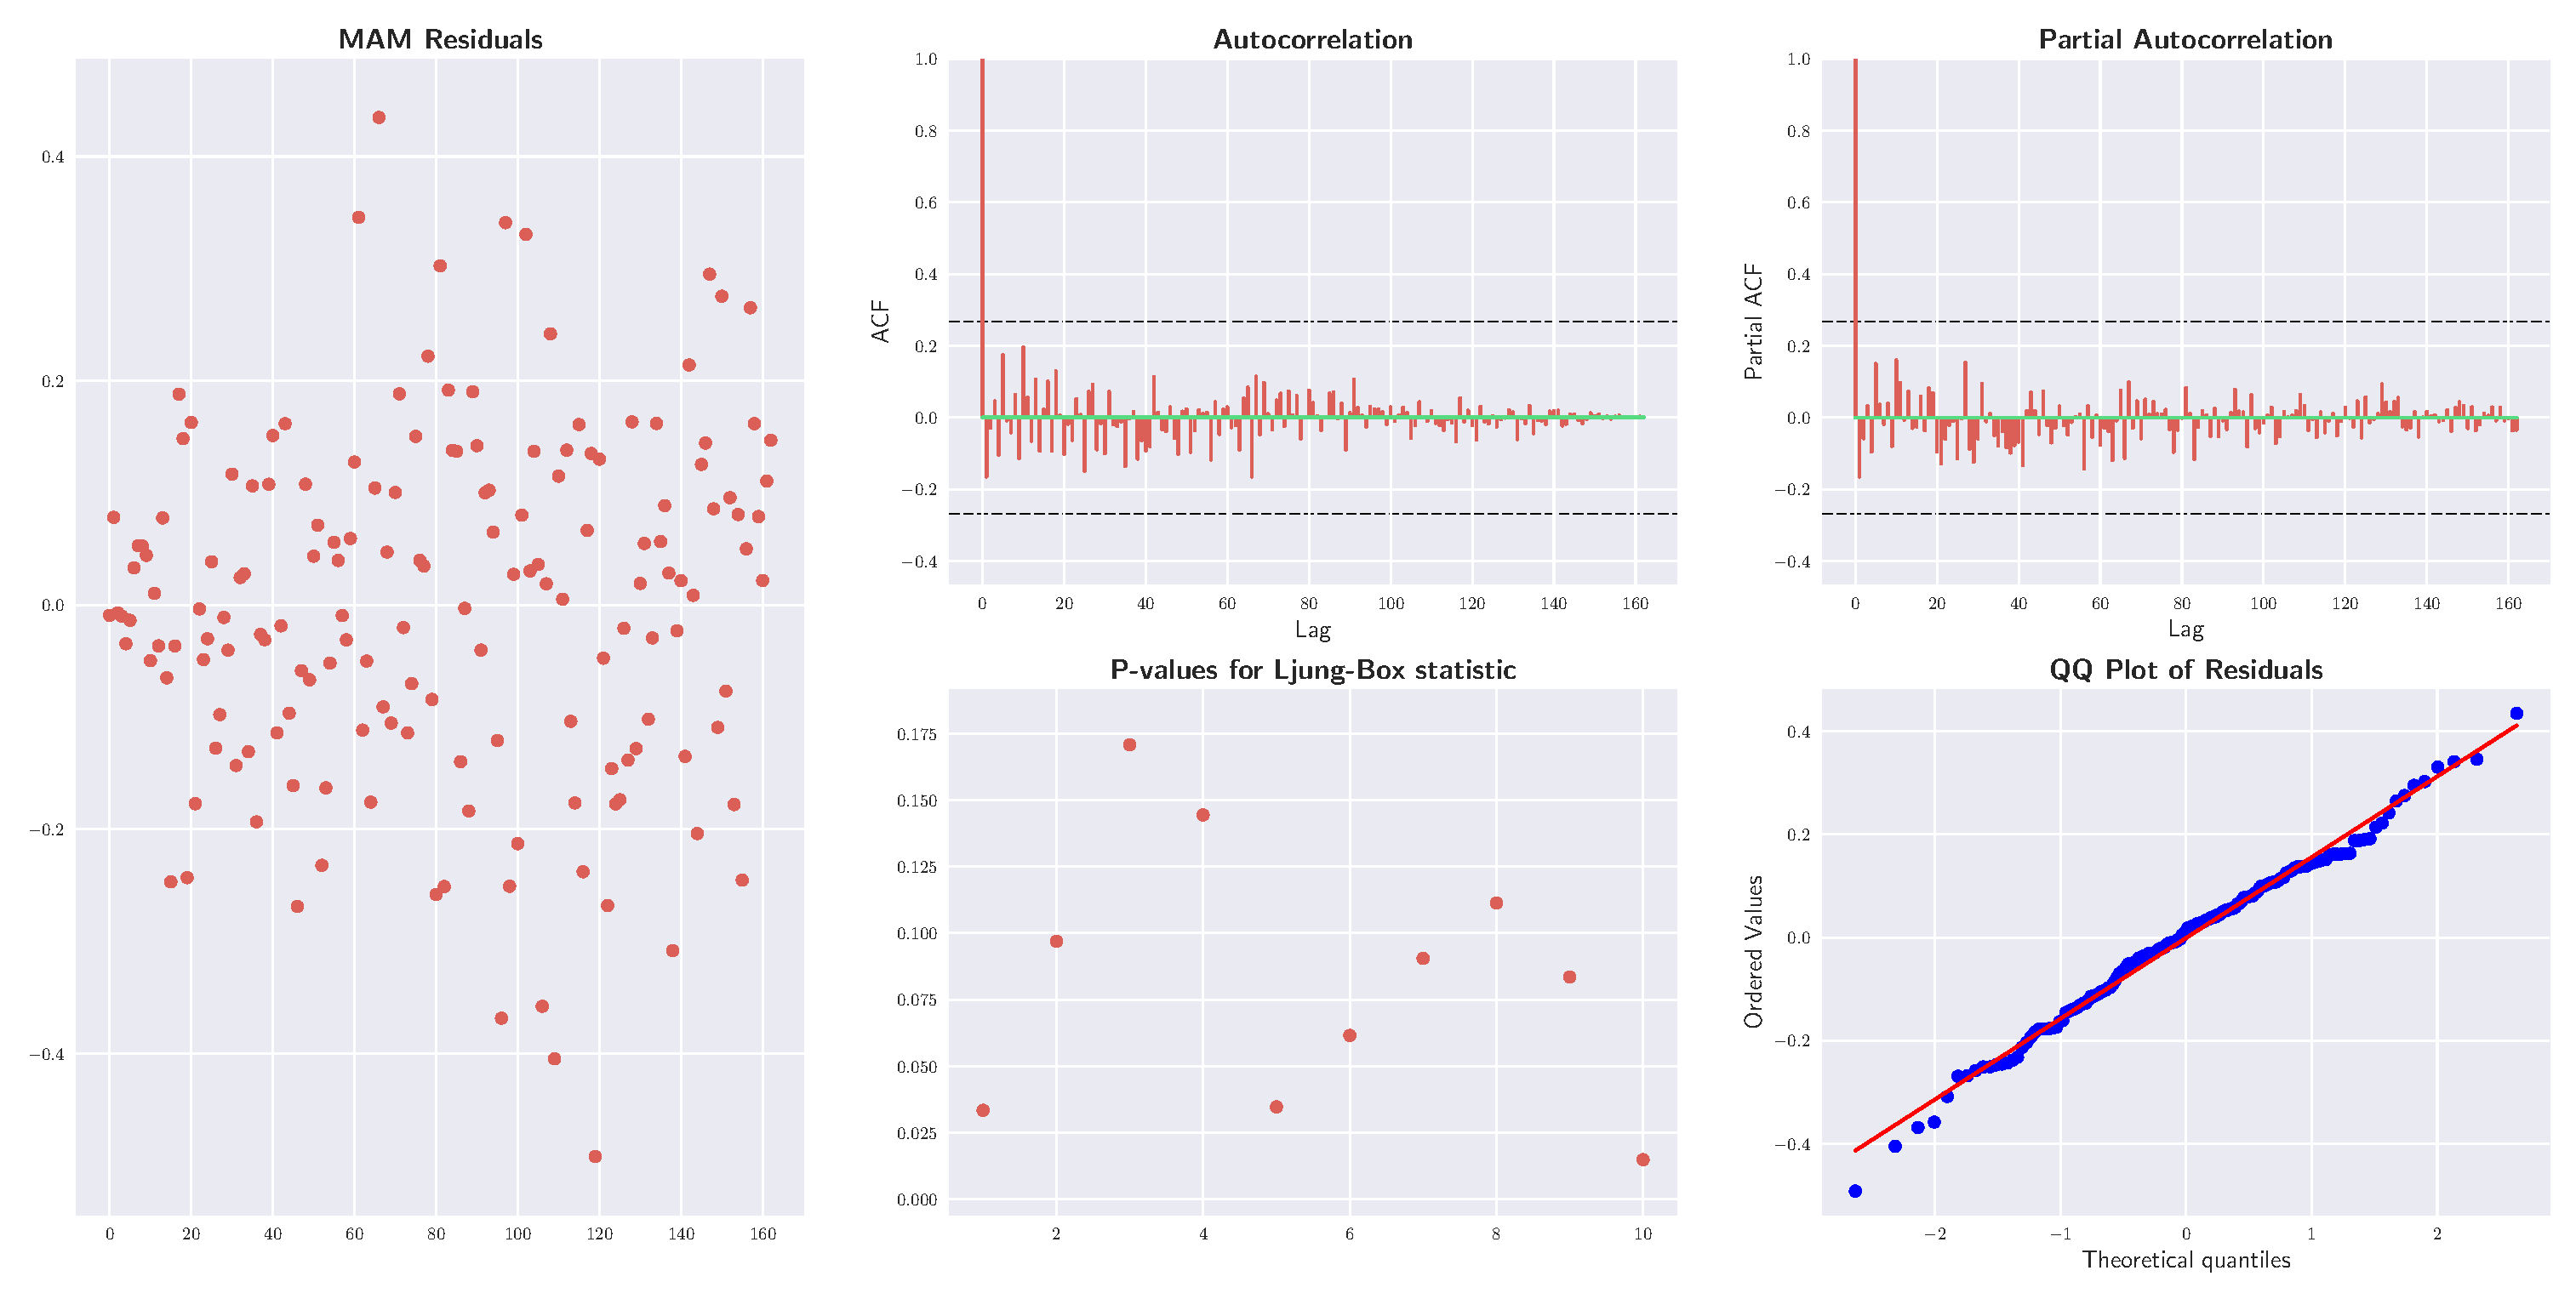
\includegraphics[scale=0.225,left]{mam_res}
		\caption{MAM residuals diagnostic tests.}
	\end{figure}
\end{frame}

\section{Conclusion}
\begin{frame}{Summary}
\begin{itemize}
\item Linear splines to determine significant changes in time, such as the 1997-1998 El Niño.
\item Regression analysis to determine a good fit for our data and to detrend the data set.
\item Determine frequency components from the estimate power spectrum to estimate the seasonality component.
\item Developed an AR(2) model from the detrended and de-seasonalized data.
\item  AR(2) model captures most of the structure for colder seasons rather than the warmer seasons.
\end{itemize}

\end{frame}

\section{Future Work}
\begin{frame}{Spatial Analysis}
Add fitting regression models to locations on the same latitude to see if there are similaritiese in the trends, change-points, and periodicities.

Exploring a two-way model, PCA + ICA, to extract certain stable patterns whose temporal trend matches physical phenomena.

\begin{figure}[!tbp]
  \centering
  \subfloat[63° latitude local.]{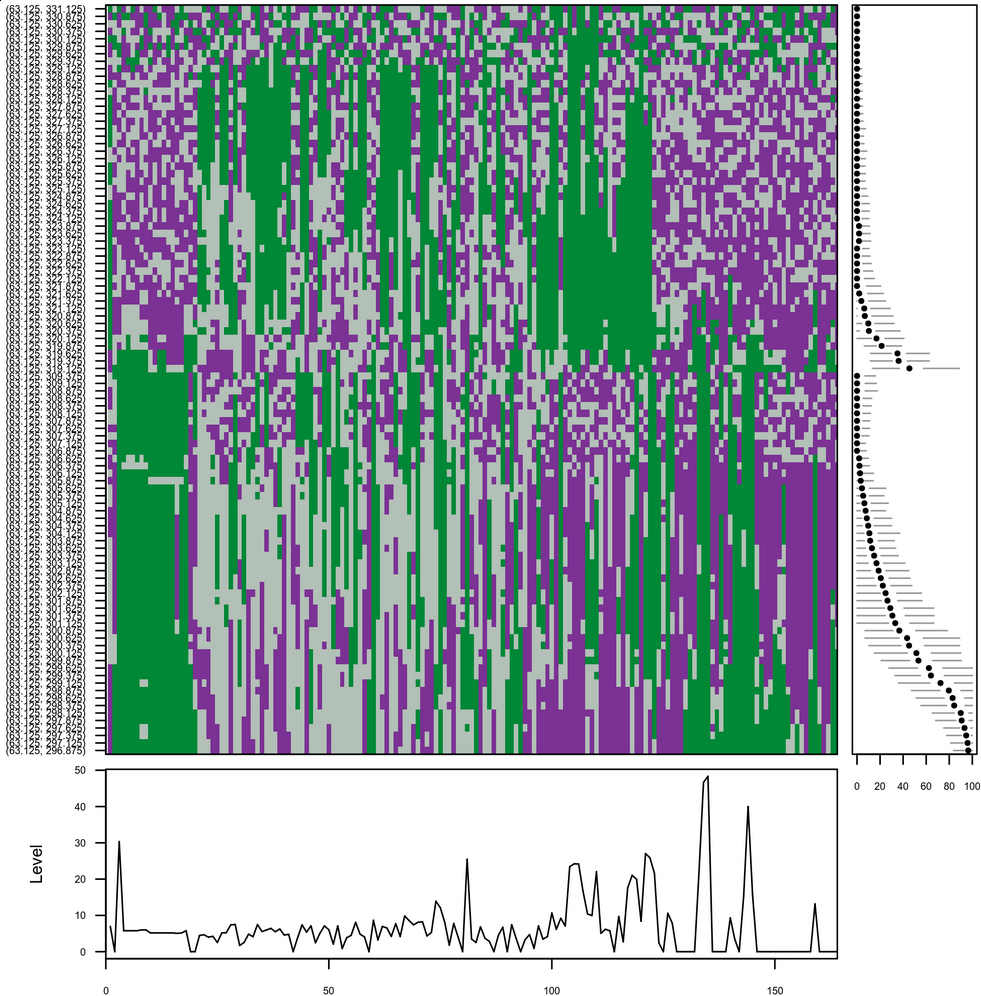
\includegraphics[width=0.34\textwidth]{lat63l}\label{fig:f1}}
  \hfill
  \subfloat[63° latitude global.]{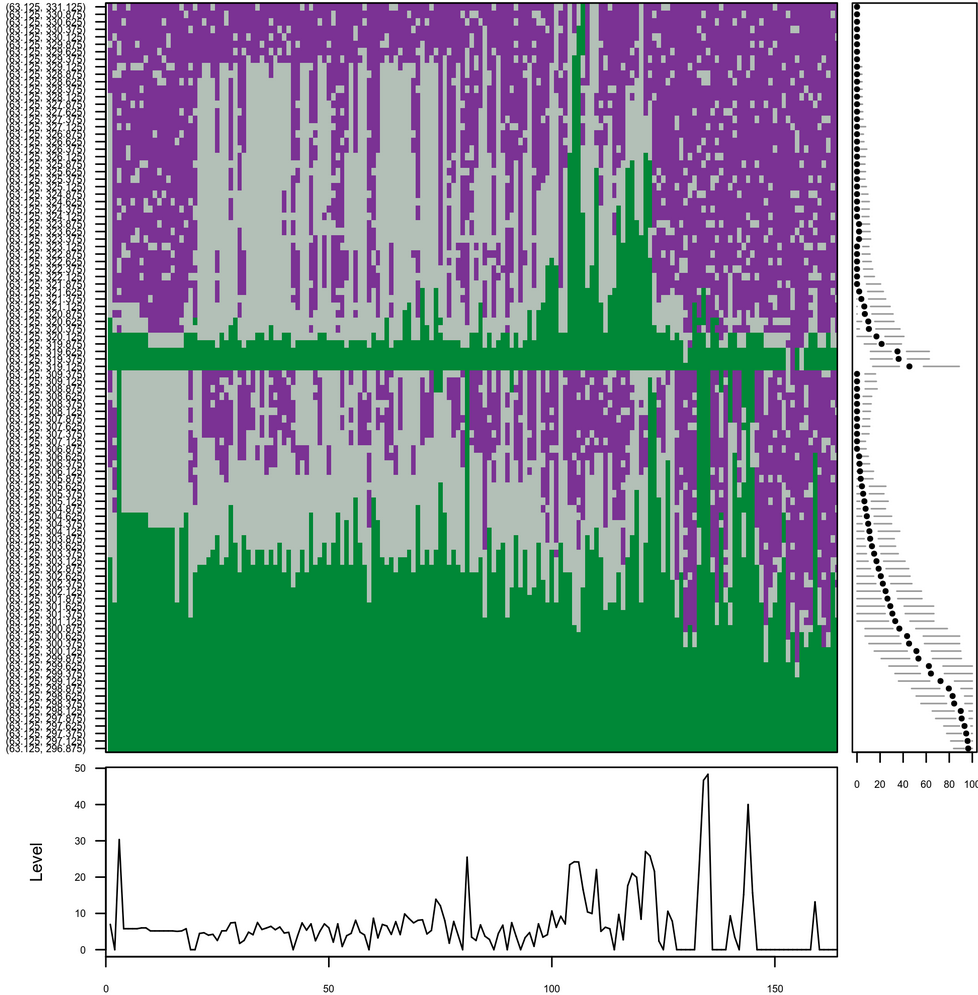
\includegraphics[width=0.34\textwidth]{lat63g}\label{fig:f2}}
  \caption{Comparison of 100 different series at 63° latitude. Green, grey, and purple indicates: high, medium, low levels of sea ice concentration, respectively.}
\end{figure}

\end{frame}

\begin{frame}{Acknowledgements}

Dr. Hernando Ombao, Ph.D. \\
\hspace{6} For acting as my advisor for this research. \\

\\
\vspace{\baselineskip}\linebreak
KAUST Visiting Student Research Program
\end{frame}


\end{document}
